% Burkhard Ritter, April 2014

\documentclass[11pt]{book}
\usepackage{amsmath,amssymb}
\usepackage{graphicx}
\usepackage{cite}
\usepackage{hyperref}
\usepackage[letterpaper]{geometry}
\usepackage{caption}
\usepackage{subcaption}
\usepackage{bm}
%\pagestyle{empty}
\begin{document}

\graphicspath{}

% TODO: title
\title{Characterizing Quantum-Dot Cellular Automata}
%\institute{Department of Physics\\University of Alberta}
\author{Burkhard~Ritter\\Supervised by Prof.~Dr.~Kevin~Beach}
\date{May 2014}
\maketitle

\tableofcontents

% http://kb.mit.edu/confluence/pages/viewpage.action?pageId=3907057
% ``LaTeX's margins are, by default, 1.5 inches wide on 12pt documents, 1.75
% inches wide on 11pt documents, and 1.875 inches wide on 10pt documents.''
% Page size for letter paper format is 8.5 by 11 inches.
% For 11pt this means the text is 8.5-2*1.75=5 inches wide.
% I am not sure why, but in gnuplot with the epslatex terminal a width of
% 6inches seems to fit best.

\chapter{Introduction}

The rise of electronic information technology has been one of the main drivers
of economical and societal change over the past seventy years. Computers have
flown us to the moon, trade stocks, diagnose illnesses, and even run simulations
of quantum spin systems. The advent of the internet, invented some 25 years ago,
and the relentless march of an army of mobile gadgets, from the venerable
notebook, over the smart phone and tablet, to wearable tech of all forms and
colours, together with readily available mobile data connections, is changing
the way we communicate, socialize, read, write and think. The benefits of
information technology are so multifaceted and ubiquitous that it is easy to
take them for granted. Yet as we ask for faster, more functionally rich, and
lighter devices, the data centres that feed us our cloud streams have developed
a great hunger for energy. And if the internet of things is supposed to happen,
it surely needs more energy-efficient devices than the phones that we always
keep in sight of a power outlet. The desire to build functional and at the same
time more power-efficient computing technology has led to efforts at all levels
of the technology stack, from the data centres, to the processor architectures,
to better and more parallel algorithms. Digital circuitry and specifically the
transistor, which underpins all of modern day information technology, have not
been an exception.

%%%%%%%%%%%%%%%%%%%%%%%%%%%%%%%%%%%%%%%%%%%%%%%%%%%%%%%%%%%%%%%%%%%%%%%%%%%%%%%%

\newacronym{QCA}{QCA}{quantum-dot cellular automata}
\newacronym{CMOS}{CMOS}{complementary metal-oxide semiconductor}
\newacronym{NMOS}{NMOS}{n-type metal-oxide-semiconductor}
\newacronym{MOSFET}{MOSFET}{metal-oxide-semiconductor field-effect transistor}
\newacronym{MEMS}{MEMS}{micro-electro-mechanical systems}
\newacronym{MEM}{MEM}{micro-electro-mechanical}
\newacronym{LED}{LED}{light-emitting diode}
\newacronym{CNTFET}{CNTFET}{carbon nanotube field-effect transistor}
\newacronym{FET}{FET}{field-effect transistor}
\newacronym{EQCA}{EQCA}{electrostatic quantum-dot cellular automata}
\newacronym{MQCA}{MQCA}{magnetic quantum-dot cellular automata}
\newacronym{NML}{NML}{nanomagnetic logic}
\newacronym{ICHA}{ICHA}{intercellular Hartree approximation}
\newacronym{ITRS}{ITRS}{International Technology Roadmap for Seminconductors}

The penetration of computing technology into all aspects of modern life has been
fuelled by the incredible success of the \cgls{CMOS} integrated circuit.
Computer chips have become ever more cheaper, smaller, power-efficient, and at
the same time much more capable. But there is a growing concern that \cgls{CMOS}
is close to its scaling limits---that it can no longer become ever faster and
cheaper. \cgls{CMOS} uses two complementary n-type and p-type \cglspl{MOSFET},
greatly reducing power consumption compared to older technologies, such as
\cgls{NMOS} logic.  Invented in the early 1960s, the \cgls{CMOS} integrated
circuit has since seen the number of transistors per chip double roughly every
two years, an exponential growth predicted by Gordon Moore and hence known as
Moore's law \cite{moore1965cramming}. Whereas in the eighties feature sizes were
on the order of micrometres, today's processors use a 22 nm process and
integrate billions of transistors on a single chip \cite{bohr2011evolution}. One
of the main reasons for the relentless miniaturization of \cgls{CMOS} technology
is cost reduction. In the manufacturing process, the cost is dominantly set per
wafer---the slab of pure crystalline silicon used as the device substrate.
Therefore, chips become cheaper by either increasing the size of the
wafer---current silicon wafers are typically 30 cm in diameter---or by
increasing the device density and thus by smaller feature sizes. Obviously,
higher device density means more functionality per same-area chip. But smaller
feature sizes also, in principle, allow for shorter switching times and reduced
switching energy, and thus faster and more power-efficient devices. In the past,
obstacles that seemed to inhibit the continued downscaling were time and again
overcome by scientific and engineering ingenuity, and the exponential growth
predicted by Moore's law has been kept pace with.  Technological innovation has
been fuelled and financed by consumer demand for more capable and functionally
rich devices.

Historically, feature size scaling was limited by the photolithographic process
used to manufacture semiconductor integrated circuits. But advances in
fabrication technology, such as 193 nm immersion lithography and double
patterning, have pushed below the 32 nm mark, with 10 nm deemed possible.
Beyond, extreme ultraviolet lithography is being developed, promising even
smaller feature sizes. These dimensions approach the atomic scale and further
downsizing is increasingly inhibited by the fundamental physical limits of the
\cgls{MOSFET}. Simply put, the smaller the transistor in size, the higher the
leakage currents. There are several leakage channels. If the distance between
source and drain becomes too small, then electrons can tunnel through the
channel region regardless of the gate barrier, and it has been estimated that
5.9 nm is the minimal gate dimension before this tunnelling current becomes
substantial \cite{cavin2012science}. Similarly, the gate voltage has to shrink
with shrinking feature sizes, which increases the subthreshold current through
the channel region. Lastly, if the gate oxide layer becomes too thin, electrons
can tunnel from the gate to the drain, again leading to a leakage current. Some
of these problems can be mitigated by technological advances. For example,
current generation microprocessors substitute the traditionally used silicon
dioxide with materials with higher relative permittivities, such as hafnium
oxide, for the gate oxide, allowing thicker oxide layers and thus decreasing
electron tunnelling. But overall, smaller feature sizes, which lead to faster
switching times and higher device densities, significantly increase leakage
currents.  Already, leakage is a substantial part of the total power consumption
of current devices.

The \cgls{ITRS} \cite{itrs2011} maps out the pace of future \cgls{CMOS}
miniaturization and estimates that feature size and voltage scaling can continue
for one or two decades, before reaching its absolute lower limit. Even with the
scaling limits approaching, \cgls{CMOS} is still a very viable technology with
several strategies for future improvements. On the \cgls{MOSFET} level,
specialized \cglspl{FET} for specific applications could be used, possibly on
the same chip. For example, if speed is paramount then transistors with short
switching times but high leakage, and therefore high power consumption, can be
employed. Conversely, for power-conscious applications, slower transistors with
larger feature sizes but less leakage would be preferable
\cite{cavin2012science}. On a higher level, architecture and circuit design
could---and this is already done to some extent---work around the changed
electronic characteristics of downscaled devices. For manufacturing, higher
parallelism in fabrication, e.g.~larger wafers, could cut down costs. More
clever packaging, for example by stacking circuits on top of each other, could
increase device density further. Lastly, the integration of different and
complementary technologies with \cgls{CMOS} directly on the chip holds
significant promise for future applications.  Combining \cgls{CMOS} circuitry
with optical devices, such as waveguides, detectors, \cglspl{LED}, and Lasers,
or radio frequency, or \cgls{MEMS}, to name just a few possibilities, would all
yield devices with richer functionality. Eventually, however, merely pushing
\cgls{CMOS} further will not be enough, and, consequently, considerable effort
has been put into the search and development of completely new computing
paradigms that could one day replace \cgls{CMOS} technology. Even if an emerging
new computing technology could not compete with \cgls{CMOS} in all aspects, it
could, conceivably, be used for specific applications, e.g.~memory, and thus
complement traditional circuitry.

%%%%%%%%%%%%%%%%%%%%%%%%%%%%%%%%%%%%%%%%%%%%%%%%%%%%%%%%%%%%%%%%%%%%%%%%%%%%%%

There is no shortage of ideas for novel computing principles and architectures
to replace or complement the existing technology \cite{cavin2012science}
\cite{bernstein2010device}. Broadly speaking, these ideas fall into three
categories. First, some device proposals seek to incrementally improve the
\cgls{MOSFET}. They might exploit better materials, or be based on other physical
principles internally, but show the same characteristics and outside
functionality as the transistor. They would be a drop-in replacement for
\cglspl{MOSFET}, and the computing architecture would remain otherwise unchanged.
Second, devices have been suggested that implement Boolean logic but use
different physical properties to store and communicate the binary state and
might, as a consequence, allow different architectural designs that better and
more efficiently exploit their specific characteristic properties. Lastly, some
ideas explore the radical departure from the existing computing architecture.
They do not necessarily strive to realize Boolean logic and include examples
such as quantum computing and neuromorphic computing, that is, computing based
on neural networks or otherwise inspired by nature \cite{mead1990neuromorphic}
\cite{schemmel2010wafer} \cite{furber2012overview}. These proposals are at
various stages of development. Some are only concepts, others have seen
extensive numerical studies, and others still have been realized experimentally.
However, none of the ideas for novel computing architectures is anywhere close
to becoming a mature technology that could rival \cgls{CMOS}, and there is also no
obvious candidate that could be pushed forward as the single most promising
future technology.

Devices implementing Boolean logic can be characterized by the physical
property---the computational variable---used to represent binary state, as well
as input and output \cite{nikonov2013overview}. For example, the \cgls{MOSFET} uses
charge on the oxide capacitor as its state variable, but voltage for input and
output. Other computational variables include electronic or atomic spin, used in
spintronic and nanomagnetic devices, position, used in some
micro-electro-mechanical approaches, or the electric dipole moment, used for
ferroelectric systems. For Boolean logic devices, binary switches with
characteristics similar to the transistor are usually required, such as gain,
non-reciprocity, i.e.~no feedback from the output to the input, and the ability
to chain the switches. Similarly, benchmarking often concentrates on switching
time and energy, as well as device density. However, if the proposed
architecture is sufficiently dissimilar to \cgls{CMOS}, then these metrics and
requirements become less applicable. As an example, the requirement of
non-reciprocity can be circumvented by introducing clocking schemes; switches
with more than two inputs could potentially perform logic operations
differently, or multiple operations at the same time.

Different materials are being explored to improve the characteristics of the
existing field-effect transistor. For example, III-V compounds such as InAs can
be used for the channel of the transistor to increase electron mobility and
hence switching speeds. Similarly, making the channel a carbon nanotube achieves
nearly ballistic transport, and these devices are then called \cglspl{CNTFET}.
As another example, tunnel-junction field-effect transistors may be used to
realize binary switches \cite{nikonov2013overview} \cite{cavin2012science}. For
most of these approaches, however, accurate and reproducible manufacturing, the
integration with silicon and, not least, the upscaling of fabrication pose
severe challenges. A different route is pursued by replacing the electronic
binary switches with micro-mechanical switches, while still using the same
conventional computing architecture. \cGls{MEM} relays are relatively slow, but
provide negligible leakage currents and are easy to manufacture, making them
attractive for ultra-low-power applications, such as environmental sensing logic
\cite{kam2011design}. Prototypical \cgls{MEM} circuits have been experimentally
demonstrated \cite{spencer2011demonstration}. Further removed from \cgls{CMOS}
circuitry are spintronic devices, which use the spin degree of freedom to encode
binary information \cite{wolf2001spintronics}. Device proposals cover a wide
range of ideas of how the spin is used, stored, and interfaced with. For
example, domain wall devices represent bits by magnetization domains in
ferromagnetic wires forming a network. The domain walls are propagated through
the wire and junctions, and other geometrical layouts implement logic functions.
The wire's magnetization can then be sensed with a magnetic tunnel junction
\cite{allwood2005magnetic}. Spin wave devices encode information in the phase of
spin waves, which interfere constructively or destructively at junctions, and
multiple signals at different frequencies can potentially be processed in
parallel \cite{khitun2005nano} \cite{kostylev2005spin}. All-spin logic devices
are yet another proposed technology that stores binary state in nanomagnets
which communicate with spin-polarized currents. For logic functionality, a
majority gate has been proposed where spin-polarized currents mix and the
majority spin polarization wins and sets the output \cite{behin2010proposal}
\cite{srinivasan2011all}. 

\cGls{QCA} is a beyond-\cgls{CMOS} computing paradigm that is a more radical
departure from conventional \cgls{CMOS} circuit design than most of the
approaches discussed so far \cite{lent1993quantum}. The binary state is encoded
as a bistable charge distribution---electric dipoles---in a cell consisting of
several quantum dots. Cells interact through electrostatic forces in a fashion
similar to a cellular automaton, where each cell's state is dominantly set by
its closest neighbouring cells. The device functionality is determined by the
geometrical arrangement of the cells. For example, cells placed next to each
other in a horizontal line can transport a signal and therefore function as a
wire \cite{lent1993lines}. Multiple input cells placed as closest neighbours to
a fourth cell vote on that cell's state, and the majority wins. This majority
gate is used to realize AND and OR logic; a different geometric arrangement
implements an inverter. \emph{A priori}, the information flow in quantum-dot
cellular automata is not directional. Rather, the computation process can be
understood as perturbing the system out of its ground state by setting external
inputs, where the device then dissipatively propagates to its new ground state,
which corresponds to the computational solution of the problem the circuit was
designed to solve. The approach is current-free and promises extremely low-power
operation. On a higher level, to design large-scale \cgls{QCA} circuits,
directionality in information flow is enforced by introducing a clocking scheme
\cite{lent1997device}. Quantum-dot cellular automata are the subject of this
thesis.

The underlying idea of \cgls{QCA}---bistable interacting cells---is quite
versatile and can be recast in different physical domains. For example, within
the last decade the possibility of molecular \cgls{QCA} implementations has been
explored \cite{lent2000bypassing} \cite{lent2003molecular}. Cells would be
comprised of molecules instead of quantum dots and these molecules have to allow
for bistable electron charge distributions. Due to their molecular scale, these
devices promise to operate at room temperature and allow extremely high device
densities.  Molecular electronics offers the prospect of efficient
self-assembly. However, a molecular \cgls{QCA} scheme also poses some severe
challenges: suitable molecules need to be identified, synthesized reliably,
attached to a surface and arranged in the desired geometric cell layout.
Interfacing input and output with more conventional electronics is likely to be
difficult. A second interesting adaptation of the \cgls{QCA} idea is in the
magnetic domain. \cGls{MQCA} \cite{cowburn2000room}
\cite{bernstein2005magnetic}, occasionally referred to as \cgls{NML}
\cite{cavin2012science}, employ bistable nanomagnets as cells which are coupled
through magnetic instead of electrostatic fields. \cGls{MQCA} works at room
temperature, promises very low power dissipation, and is non-volatile. Lines of
cells, the majority gate, and clocking have all been demonstrated experimentally
\cite{imre2006majority} \cite{alam2007clocking} \cite{alam2012chip}.

For the original \cgls{QCA} scheme---sometimes referred to as \cgls{EQCA} to
distinguish it from the molecular and magnetic variants---a number of systems
have been explored for experimental implementation. Lent \emph{et al}.\
demonstrated the first experimental \cgls{QCA} cell in 1997 in a metal-island
system \cite{orlov1997realization}. The quantum dots were realized as
tunnel-coupled aluminum islands of micrometer size at millikelvin temperatures,
and the bistable nature of the cell was observed.  Experiments were then
extended to demonstrate binary wires (two cells), majority gate operation (a
single cell with three inputs), and a shift register (consisting of six dots)
\cite{orlov1999experimental} \cite{amlani1999digital}
\cite{kummamuru2003operation}. Single \cgls{QCA} cells have also been
implemented in GaAs\,/\,AlGaAs heterostructures, ion-implanted phosphorus-doped
silicon, and, most recently, on a hydrogenated silicon surface
\cite{gardelis2003evidence} \cite{mitic2006demonstration}
\cite{haider2009controlled}. On the hydrogenated silicon surface, individual
hydrogen atoms are removed with a scanning tunnelling microscope tip. The
remaining dangling bonds act as quantum dots.  These atomic silicon quantum dots
are tunnel-coupled when placed close enough together (a few nanometers), at
larger distances they interact only via Coulomb repulsion
\cite{pitters2011tunnel}. This silicon-based \cgls{QCA} implementation is
particularly exciting, because it promises room temperature operation due to its
small feature sizes and large electrostatic energy scales, and potentially easy
integration with the existing \cgls{CMOS} technology. The precision and
upscaling of the fabrication capabilities have seen encouraging progress
recently \cite{wolkow2013silicon}.

%%%%%%%%%%%%%%%%%%%%%%%%%%%%%%%%%%%%%%%%%%%%%%%%%%%%%%%%%%%%%%%%%%%%%%%%%%%%%%

On the theoretical side, the building blocks of \cgls{QCA} circuitry, such as
the single cell or a line of cells, have been characterized and the dynamical
behaviour of larger systems such as gates has been studied \cite{lent1993lines}
\cite{tougaw1996dynamic}. Importantly, the cell-cell response---the switching
behaviour of a cell with respect to an input cell---was found to be non-linear
and exhibit gain, two of the main requirements for building traditional
\cgls{CMOS}-like integrated logic circuits. If that is indeed true, then lines
of cell are always fully switched and fanout and concatenation of devices do not
pose difficulties.  Clocking schemes have been introduced to improve the
reliability and speed of \cgls{QCA} computations and, starting from the basic
building blocks, more complex circuits like shift registers, adders, and memory
have been explored \cite{lent1997device} \cite{hennessy2001clocking}
\cite{rahimi2008quantum}. A circuit design and simulation program exists, which
treats the \cgls{QCA} system with a high level of abstraction and strongly
idealized cells \cite{walus2004qcadesigner}.

Numerical work on \cgls{QCA} typically starts from an extended Hubbard model.
However, because the full quantum mechanical problem becomes computationally
intractable very quickly even for small systems, two ubiquitous approximations
are employed: the \cgls{ICHA} and the two-state-per-cell approximation
\cite{lent1993quantum} \cite{tougaw1996dynamic}. Crucially, even though there
are plausibility arguments to motivate their use, neither of these
approximations has been rigorously validated. The \cgls{ICHA} approximation in
particular is problematic: as a mean field scheme \cgls{ICHA} should be expected
to over-emphasize charge-density-wave order in low-dimensional structures and
therefore potentially yield results that are too optimistic regarding the
operational range of the devices. To our knowledge, almost all previous efforts
to characterize \cgls{QCA} building blocks rest on \cgls{ICHA}, and there is a
danger that the whole emerging physical picture of the \cgls{QCA} approach is
coloured by the particularities of this mean field approximation. Recently,
Taucer \emph{et al}.~explicitly identified the need to go beyond the \cgls{ICHA}
approximation \cite{taucer2012consequences}.  Concentrating on system dynamics,
they showed that \cgls{ICHA} yields quantitatively and qualitatively wrong
results. \cGls{QCA} was found to be more fragile than previously predicted.
Although it has been argued that in practical systems, quantum decoherence would
stabilize \cgls{QCA}, the fact remains that the approximation underlying most
theoretical work on \cgls{QCA} is not well understood and known to be
qualitatively wrong in some cases \cite{blair2013environmental}.

In this work we undertake a thorough and rigorous numerical study of the
electrostatic \cgls{QCA} approach. We do not attempt the quantitatively accurate
modelling of a specific material system, but aim for the generic, semi-realistic
description of \cgls{QCA} devices. Starting from the extended Hubbard model and
using exact diagonalization, we do away with the \cgls{ICHA} approximation.
Instead, we introduce two controlled Hilbert space truncations, the fixed-charge
and the bond model, whose limits we study and understand. We derive the
two-states-per-cell model---which is equivalent to a transverse-field Ising
model---and show the limits in which it is an appropriate description of
\cgls{QCA} systems. Restricting ourselves to time-independent properties, we
concentrate on a few simple building blocks of \cgls{QCA}---the cell and a line
of cells---but aim to characterize them in as detailed and unbiased a way as
possible. Remarkably, even for these very simple \cgls{QCA} systems, we already
find notable differences to previously published results. In particular, the
cell-cell response is \emph{linear} and does not exhibit gain. This has profound
consequences and essentially changes the whole physical picture of \cgls{QCA}.
We explore the systems' characteristics over a wide range of parameters and
establish minimal requirements for \cgls{QCA} operation as well as parameters
for optimal performance.  Using the two-states-per-cell model in a tightly
controlled parameter regime, we briefly investigate wires of up to twelve cells
in length and the majority gate.

The following chapter introduces the \cgls{QCA} approach in detail. We explain
the basic idea, logic gates as the building blocks of \cgls{QCA} circuitry, and
the clocking of larger devices. As an example experimental system, we discuss
atomic silicon quantum dots, which we use as a reference throughout the thesis.
We then dive into the modelling of \cgls{QCA} systems, and specifically the
extended Hubbard model which we use as our starting point. Previous theoretical
results are presented, along with a more detailed explanation of the
intercellular Hartree approximation. We conclude the chapter with a brief
overview of our exact diagonalization implementation.
Chapter~\ref{ch:approximations} focuses on the approximations we use. Two
Hilbert space truncations are introduced, the fixed-charge model and the bond
model. We then derive an Ising-like model---the two-states-per-cell
approximation---as an effective low-energy model from the bond Hamiltonian. This
derivation will already yield some insights into the characteristics of the
\cgls{QCA} paradigm. The last part of the chapter goes into great detail to
understand how the approximations work and in which regime they are valid. The
fourth chapter presents the numerical results from our study. We use a
three-cell wire as an exemplary \cgls{QCA} system to investigate its basic
characteristics. We then employ an extended ``cluster'' mean field scheme in an
effort to establish lower boundaries for workable \cgls{QCA} system parameters.
Using the Ising model for lines of up to twelve cells, we identify a set of
parameters where the \cgls{QCA} approach works well and put those parameters
into context by contrasting them with corresponding parameter estimates for the
atomic silicon quantum dots. The chapter concludes with a brief numerical
exploration of the majority gate. The last chapter summarizes our results and
offers a perspective on future directions for research on the \cgls{QCA}
approach.

\chapter{Quantum-dot cellular automata}
\label{ch:QCA_intro}
\graphicspath{{../gfx/chapter01/}}

\section{An alternative computing paradigm}
\label{sec:an_alternative_computing_paradigm}

\begin{figure}
  \center
  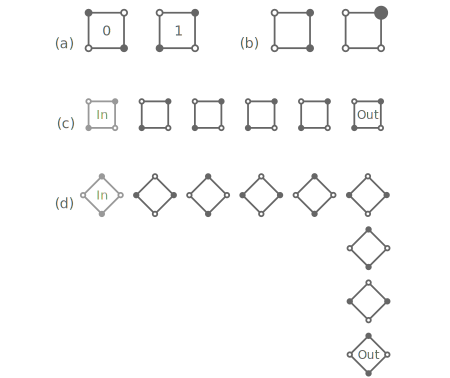
\includegraphics{intro_qca}
  \caption
[Building blocks of quantum-dot cellular automata (QCA) circuitry]
{
Building blocks of quantum-dot cellular automata (QCA). (a) A QCA cell consists
of four quantum dots on the corners of a square and is occupied by two
electrons. Due to Coulomb repulsion, two energetically preferred states emerge,
logic 0 and logic 1. (b) Both electrons occupying the edge of the cell or
doubly occupying a single quantum dot are unfavourable high-energy states. (c) A
straight line of cells functions as a wire and transmits a signal. (d) A
diagonal line of cells (cells rotated by $45^{\circ}$) transmits a signal
alternating from cell to cell. Wires can have kinks.
}
  \label{fig:intro_qca}
\end{figure}
%
\begin{figure}
  \center
  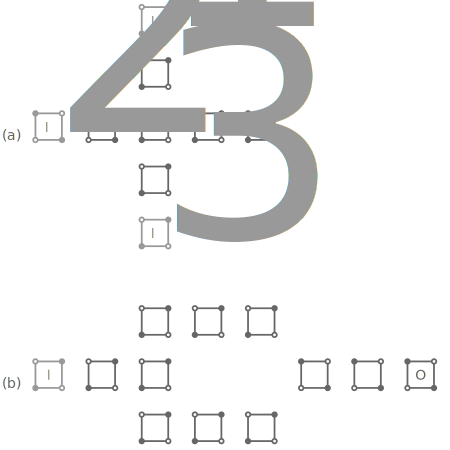
\includegraphics{gates}
  \caption
[QCA gates]
{
QCA gates. (a) The majority gate's three inputs ``vote'' on the output. The gate
is commonly operated with one fixed input, for example $I_3$, and then functions
as an AND ($I_3 = 1$) or OR gate ($I_3 = 0$) for the remaining two inputs. Here
the gate performs the computation $1 \land 0 = 1$. (b) The inverter performs
logical negation, swapping logic 0 for logic 1 and vice versa.
}
  \label{fig:gates}
\end{figure}

Lent \emph{et~al}.\ introduced the concept of quantum-dot cellular automata as
an alternative computing paradigm in 1993 \cite{lent1993quantum}. They devised a
novel physical scheme to build digital circuits that would overcome some of the
limitations of complementary metal-oxide semiconductor (CMOS) technology,
promising potentially lower power consumption, higher device density, and faster
clocking. As the name suggests, quantum-dot cellular automata (QCA) are made
from quantum dots that are grouped into cells. Figure~\ref{fig:intro_qca}(a)
shows a basic QCA cell in which four quantum dots are arranged on the corners of
a square. The dots are idealized as highly localized single orbitals that are
perfectly decoupled from some non-intrusive medium or substrate.  Because of the
Pauli principle, each dot can be occupied by zero, one, or two electrons. In the
QCA scheme, however, each cell is occupied by exactly two electrons, and each
constituent dot is quarter-filled on average. The electrons tunnel only weakly
between different dots in a cell, and the dominant energy scale is the Coulomb
repulsion between the particles. Because of the large energy cost to two
electrons occupying the same site or adjacent ones, the diagonal states are the
two energetically preferred electron configurations. In comparison, edge states
or doubly occupied quantum dots are unfavourable higher energy states, see
Fig.~\ref{fig:intro_qca}(b). The two diagonal states can be identified with
logic 0 and 1, respectively. \emph{A priori} the two bit encodings have the same
energy, but this degeneracy can be lifted by an external Coulomb potential,
arising, for example, from a second nearby QCA cell.

A single cell by itself is not very interesting. But multiple cells can be
positioned next to one another, for example as a straight line of cells, as
shown in Fig.\ref{fig:intro_qca}(c). The approach once again assumes that
Coulomb forces are strong and that electron tunnelling between cells is very
small. For a straight line of cells, the long-ranged, unscreened Coulomb forces
will tend to align the electron configurations of adjacent cells. If the first
cell is in logic state 1, then the second cell will also prefer logic state 1
and so in turn will all the other cells in the line. The situation is the same
for logic state 0. Therefore, a straight line of cells is similar to a wire not
only in geometry, but also in functionality: it transmits a digital signal. The
same is true, with slight modifications, for a diagonal line of cells---cells
rotated by $45^{\circ}$, as illustrated in Fig.~\ref{fig:intro_qca}(d). In this
case, the signal alternates from cell to cell; that is, logic 1 will follow
logic 0 which followed from logic 0, and this again is simply by virtue of the
dominant Coulomb interaction between electrons on different cells. By using an
even number of cells the diagonal line of cells works as a wire just as well as
a straight line of cells. The pictogram also demonstrates a $90^{\circ}$ kink
for the diagonal line of cells, which our newly gained intuition for these
Coulomb-driven systems expects to pose no problem for signal transmission.

The main idea of the QCA approach becomes apparent: ideal, bistable cells
interact with each other solely by Coulomb repulsion. By arranging the cells in
clever geometries, we can realize interesting functionalities. The idea as such
is quite general and does not strictly rely on the two-electron--four-dot cell
introduced above. Indeed, a number of variations exist, such as cells consisting
of two dots and occupied by only one electron that interact via dipole fields
instead of quadrupole fields as for the conventional cells. Another variation is
a four-dot cell with six electrons---two holes---instead of two electrons. Even
the interaction need not be Coulombic. For example, magnetic QCA schemes have
been explored \cite{bernstein2005magnetic}. While QCA carries ``quantum'' in its
name and is sought to be implemented at the nanoscale, the approach operates
close to the classical limit. The Coulomb interaction dominates with the
tunnelling of electrons serving as a small perturbation, which nonetheless
drives the system's dynamics. The approach is insensitive to the spin degrees of
freedom. Let us finally note that QCA is a not a cellular automata in a strict
mathematical sense, but only by analogy to the idea of cells evolving according
to simple rules that depend on neighbouring cells.

One clever geometrical cell arrangement, the majority gate, is shown in
Fig.~\ref{fig:gates}(a). The gate has three inputs which ``vote'' on the
central cell. The majority wins and sets the single output. The device is
commonly operated with one fixed input, for example $I_3 \doteq 0$ or $I_3
\doteq 1$. In the first case, with $I_3 \doteq 0$, the device functions as an
AND gate for the remaining two inputs, $O = I_1 \land I_2$. In the second case,
with $I_3 \doteq 1$, it is an OR gate with $O = I_1 \lor I_2$. The figure shows
the gate performing the computation $1 \land 0 = 1$. Now the only missing piece
for Boolean algebra is negation, $O = \lnot I$. We had already seen that simply
arranging cells at an $45^{\circ}$ angle as in the diagonal line of cells
negates the signal from cell to cell. The inverter, shown in
Fig.~\ref{fig:gates}(b), recasts this idea into a more robust layout. With
that we have, at least in principle, all the necessary building blocks for
Boolean algebra and thus digital circuitry.

Conceptually, it is most elegant to set the inputs for a QCA circuit via driver
cells---cells that resemble the QCA cell in form, but are made up of static
point charges instead of quantum dots. These static charges are thought to be
manipulable to vary the input smoothly from the logic 0 to the logic 1 state.
In Figs.~\ref{fig:intro_qca}~and~\ref{fig:gates}, these driver cells are
represented in light grey. Of course, in practice such driver cells would be
difficult if not impossible to implement and the inputs are more likely set by
leads that provide the necessary perturbative electrostatic fields. The output
of a QCA device can be directly read from its output cells. In practical
implementations this will require a non-trivial charge probing apparatus.
Changing the input for a QCA device throws the system into an excited,
non-equilibrium state. The system will then dissipatively propagate to its new
ground state. For the given inputs, this ground state corresponds to the
solution of the computational problem the circuit is designed to solve. Let us
emphasize this: in QCA, the computational solution maps directly to the physical
ground state. While the computation is being performed, only a few charges move locally,
in each cell. Operating close to the ground state, QCA is thus a truly
current-free approach and consequently inherently low-power, especially when
compared with CMOS technology. But the operation close to the ground state also
raises concerns for the operational temperature for these devices. It is clear
that for real-world applications we would want to engineer the system so that
the energy gap between the ground state and the low-lying excited states far
exceeds room temperature. Different material systems provide different
dissipative channels, and modelling them quantitatively or even qualitatively
correctly is very challenging. As a consequence, it is difficult to derive
general expectations for the clocking speed of QCA circuits. The switching speed
of a majority gate, for example, will greatly depend on the system's parameters,
but particularly on the nature of the dissipative coupling of the circuit to its
environment. A small dissipative coupling will have the output polarization
oscillating before it eventually settles to its correct value. A very
dissipative system in contrast might get stuck in meta-stable states. 

QCA circuits consist of wires, gates, and other structures arranged on a
two-dimensional surface---very similar to conventional electronics devices.
However, the structures themselves are quasi-one-dimensional, and this poses a
challenge for building large-scale QCA circuits. A good example is a single long
wire, which is truly one-dimensional. When we think about switching the input
for the wire, we think of the information being propagated as a charge density
wave along the line of cells, or, equivalently, as propagating the domain
boundary between logic 0 and logic 1. This domain boundary incurs an energy cost
that the system seeks to minimize, causing the wire to order. For an
increasingly longer wire, however, the gain in entropy for moving a domain
boundary freely throughout the wire ($S \sim \log N$, $N$ the number of cells)
soon exceeds the loss in energy, which is reflected by the free energy of the
system ($F = U - T S$). Quite generally, a one-dimensional system with discrete
(rather than continuous) degrees of freedom cannot be ordered in the
thermodynamic limit except at zero temperature. Therefore, the
finite-temperature, infinitely long wire will always exhibit exponentially
decaying bit correlations and thus be unable to transmit a signal. The gap
between the first excited state---with two domains---and the completely ordered
ground state, together with the desired operational temperature will determine
the maximum system size.

\begin{figure}
  \center
  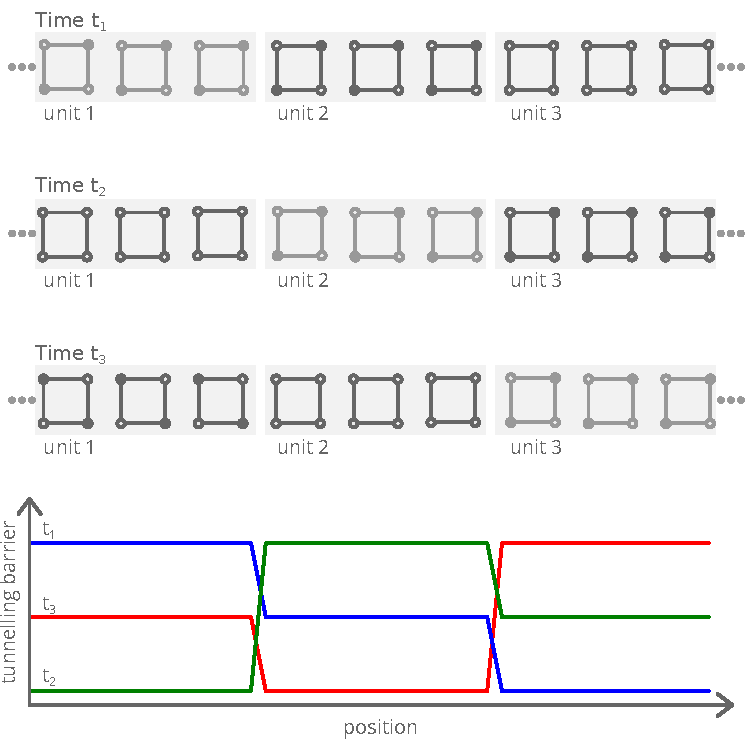
\includegraphics{clocking}
  \caption
[Clocked QCA for a line of cells]
{
Clocked QCA for a line of cells. To avoid entropy-induced disorder in large QCA
circuits, the system is partitioned into smaller units, labelled 1, 2, and 3 in
this example. By varying the tunnelling barriers, each unit is put through the
three phases \emph{frozen} (high barrier, light grey cells), \emph{active}
(medium barrier, dark grey cells), and \emph{delocalized} (low barrier, dark
grey cells with empty dots). Synchronizing the phases of adjacent units allows
to pipeline information flow and computations. The line of cell's three units
and their tunnelling barriers are shown at three different times, $t_1<t_2<t_3$.
A logic 1 state is propagated from the left to the right. At $t_3$ a logic 0
state is coming in from the left.
}
  \label{fig:clocking}
\end{figure}

To address this scaling problem, we partition large circuits into smaller units.
The size of each unit is chosen to be small enough to avoid entropy-induced
disorder at a given operational temperature. Each unit can be turned ``on'' and
``off'' separately: ideally, individual gates would allow one to effectively
raise and lower the tunnelling barriers between quantum dots in each unit and
thus provide a mechanism to freeze or delocalize the electrons. A unit with
\emph{frozen} electrons can serve as the input for a unit with more
\emph{active} charge carriers, which works like a regular QCA circuit. A unit
with completely \emph{delocalized} electrons, in contrast, will not influence
adjacent units. By putting each unit through the three phases
\emph{delocalized}, \emph{active}, and \emph{frozen} and synchronizing adjacent
units appropriately, we can control the information flow through the system very
nicely, as illustrated in Fig.~\ref{fig:clocking}. Therefore, by partitioning
the circuit and introducing a clocking scheme, we not only handle the scaling
problem but also arrive at a pipelining architecture. If and how the
tunnelling barriers can be effectively modified will depend on the details of
the specific QCA implementation. Also, in practice the QCA circuit units cannot
be too small as they must be individually addressable. Gates which turn QCA
units ``on'' and ``off'' provide another potential benefit as well. We are able
to control how and especially how fast the gate voltage is changed and should be
able to tune it with respect to the inherent time scales of the QCA system,
which are set by the system's parameters and the dissipative coupling to its
environment. This should afford a better control over the dynamics of the
switching process and might help mitigate problems such as oscillating outputs
and meta-stable states, mentioned above \cite{lent1997device}.


\section{Atomic silicon quantum dots}
\label{sec:atomic_silicon_quantum_dots}

\begin{figure}
  \center
  \includegraphics{silicon}
  \caption
[Atomic silicon quantum dots]
{
Atomic silicon quantum dots are \emph{dangling bonds} (DBs) on a hydrogenated
(100) silicon surface. (a) A scanning tunnelling microscope (STM) image of an
atomic silicon quantum dot QCA cell. (b) Band diagram of a DB on a strongly
n-doped silicon substrate. (c) The reconstructed (100) hydrogenated silicon
surface, showing dimer rows. (d) Two closely spaced tunnel-coupled DBs perturbed
by a third DB. The top right DB is seen to be more negatively charged than the
other DB of the closely spaced pair, due to Coulomb repulsion from the
perturbing third DB in the bottom left. All STM images and \emph{ab initio}
estimates from Wolkow \emph{et~al}.\ \cite{wolkow2013silicon} \cite{pitters2011tunnel}.
}
  \label{fig:silicon}
\end{figure}

Our objective is the general, rather than implementation-specific,
characterization of the QCA approach. Even so, it is still important to consider
concrete experimental realizations, not only as a motivation for our work, but
also to put our modelling and results into context. One of the most promising
and recent experimental implementations of QCA is based on atomic silicon
quantum dots, and we will therefore use them as our experimental reference.
Atomic silicon quantum dots were first demonstrated as a possible QCA
implementation by Wolkow \emph{et~al}.\ in 2009, when the group first
constructed a
single QCA cell. Figure~\ref{fig:silicon}(a) shows a scanning tunnelling
microscope (STM) image of their device. Since then impressive advances have been
made both in the understanding of the electronic properties of these quantum
dots as well as in the precise fabrication of larger QCA structures. With
atomic-scale feature sizes, this experimental system promises room temperature
operation, while at the same time tapping into the established and highly
sophisticated silicon technology. Being based on silicon should also ease
integration with existing CMOS circuitry.

Atomic silicon quantum dots are \emph{dangling bonds} on a hydrogen-terminated
$(100)$ silicon surface. Atoms on a $(100)$ silicon surface have two unsatisfied
bonds. Pairs of surface atoms form dimers, satisfying one bond. The remaining
bond is satisfied by passivating the surface with hydrogen.
Figure~\ref{fig:silicon}(c) shows a STM image of the reconstructed silicon
surface, where the dimer rows are clearly visible and the dimensions are
indicated. By applying a relatively large current through the STM tip,
individual hydrogen atoms can be removed, with atomic precision. This leaves a
\emph{dangling bond} (DB) that acts as a quantum dot: energetically, electrons
on the DB orbital sit in the silicon band gap and are therefore decoupled from
the silicon substrate. Figure~\ref{fig:silicon}(b) shows the band diagram of a
DB on an n-doped substrate. Chemically, DBs have proven to be surprisingly
robust with respect to environmental molecules. From \emph{ab initio}
calculations it is known that the sp$^3$ DB orbital extends predominantly into
the bulk and only a little into the vacuum. The orbital's lateral extent is on
the order of 1~nm and therefore spans multiple silicon lattice atoms. Due to
orbital overlap, closely spaced DBs are tunnel-coupled. A neutral DB consists of
the positive silicon ion and one electron. In the experimentally common strongly
n-doped system, the DB accepts one more electron and is therefore $-1e$
negatively charged. Conversely, in a p-doped sytem the DB will donate its
electron and become $+1e$ positively charged. The Coulomb repulsion between
negatively charged DBs can be used to adjust the filling of DB assemblies simply
by controlling the DBs' positions. For example, on an n-doped substrate two DBs
may eject one electron (which goes back to the bulk) and share the remaining
single electron, when placed close enough together. To prove this, a third DB is
placed close by, but not close enough to be tunnel-coupled. The effect of the
Coulomb repulsion can be seen via STM imaging, Fig.~\ref{fig:silicon}(d),
where the DB farthest from the perturbing external charge is more negatively
charged (darker in the STM image) than the closer DB. The observed charge shift
is only possible when both closely-spaced DBs share a single electron. To form
the previously shown QCA cell, Fig.~\ref{fig:silicon}(a), on a strongly
n-doped silicon substrate four DBs are brought close enough together so that two
electrons go back to the bulk, leaving the cell with six electrons (two holes)
in total and a cell net charge of $-2e$, which is the right charge regime for
QCA.

Atomic silicon quantum dots provide some examples of how a real world system
might be different from the idealized picture we typically employ to describe
the QCA approach. We like to think of quantum dots as highly localized orbitals.
But in the silicon system the orbitals of the DBs actually span multiple lattice
sites and only if the DBs are placed far enough apart might we still be able to
consider them as localized. We do not consider the substrate but treat quantum
dots as perfectly isolated entities. Of course, in practice the substrate will
certainly influence the QCA device. In the silicon system, free charge carriers
will screen the long-ranged Coulomb interactions that the QCA scheme relies on,
although likely on scales larger than the circuit feature size. The screening is
not necessarily disruptive for QCA and might even be beneficial, for example by
minimizing charge buildup in large systems. But to quantify the screening
accurately it is necessary to thoroughly understand and precisely model the
system; for atomic silicon quantum dots, which live at the surface, that would
surely be very challenging. The silicon substrate could also, conceivable,
provide a second tunnelling channel between DBs. In addition to electrons
hopping directly from DB to DB they could first tunnel from DB to substrate and
then back to another DB.  Therefore an accurate model for atomic silicon quantum
dots might need to accommodate the nature of the DB orbitals, screening,
multiple tunnelling channels, and possibly other effects.


\section{The extended Hubbard model}

QCA systems are typically modelled by an extended Hubbard Hamiltonian. The
Hubbard model originated in the early 1960s to describe rare-earth systems with
highly localized d- and f-electrons and has since then, of course, become one of
the most widely studied and successful models in condensed matter physics
\cite{Hubbard1964}. In basing our description on the Hubbard model we already
put some key assumptions in place. For example, we assume that the quantum dots
are similar to the highly localized d-orbitals. As discussed above, depending on
the particular QCA implementation this might or might not be a good description.
However, our interest is not in the precise details of any particular material
system; rather, our aim is to investigate universal characteristics of QCA systems.
As long as a QCA system can be broadly qualitatively described by Hubbard
physics---and most prospective QCA implementations fall into this category---our
modelling and findings should be valid. Conversely, for implementations that are
decidedly not Hubbard-like, our results might not be applicable. An idealized
but semi-realistic description is what we want and for that the Hubbard model is
indeed an appropriate---and tractable---starting point. Specifically, the
Hamiltonian we use is
\begin{equation}
\begin{split}
  \label{eq:H_QCA}
  H =
    &- \sum_{ij\sigma} t_{ij} \, c^{\dagger}_{i\sigma} c_{j\sigma}
    + U \sum_i n_{i\uparrow} n_{i\downarrow}
    - \mu \sum_{i\sigma} n_{i\sigma} \\
    &+ \sum_{i<j} V_{ij} \left( n_{i\uparrow} + n_{i\downarrow} - q \right) 
                        \left( n_{j\uparrow} + n_{j\downarrow} - q \right) \, ,
\end{split}
\end{equation}
where $c^{\dagger}_{i\sigma}$ ($c_{i\sigma}$) creates (annihilates) an electron
on quantum dot $i$ with spin $\sigma$ and the particle number operator is
$n_{i\sigma} = c^{\dagger}_{i\sigma} c_{i\sigma}$. The overlap integral between
dots $i$ and $j$ is denoted by $t_{ij}$, $U$ is the Hubbard on-site Coulomb
repulsion, $\mu$ the chemical potential, and $V_{ij}$ the long-ranged Coulomb
interaction, which is characteristic for QCA systems. For simplicity the Coulomb
term is chosen to be $V_{ij} = \frac{1}{r_{ij}}$ where $r_{ij}$ is the distance
between the two dots $i$ and $j$. We also introduce the \emph{compensation
charge} $q$ which is thought to represent a possible positive ion at each
quantum dot site. This constant positive charge allows us to tune the net cell
charge. For two electrons per cell, for example, $q=0$ yields a net cell charge
of $-2e$ whereas $q = \frac{1}{2}$ represents zero net cell charge. The $q =
\frac{1}{2}$ charge neutral cells are perfect electrostatic quadrupoles.

The geometric layout of the QCA system and therefore its functionality is
encoded in the hopping parameter $t_{ij}$ and the long-ranged Coulomb term
$V_{ij}$. For the hopping parameter, we usually only consider nearest-neighbour
hopping $t$ and specifically no hopping between the cells. While this constraint
is not strictly necessary for QCA, it is in line with the approach's underlying
idea and greatly simplifies calculations. Because the overlap integral decays
exponentially with distance, as long as the distance between dots from different
cells is larger than the distance between dots within one cell, the assumption
will introduce only a small error. Still, this is something to keep in mind if
we place cells very close to each other. Note that without inter-cell hopping we
can decompose the Hamiltonian into purely Coulombic cell-cell interaction terms
$H^{cc}_{kl}$ and single cell terms $H^c_k$, which capture the kinetics as well
as the inside-cell Coulomb interactions,
\begin{equation}
  \label{eq:H_cell}
  H = \sum_k H^c_k + \sum_{k<l} H^{cc}_{kl} \, ,
\end{equation}
where $k$ and $l$ number the cells. 

\begin{figure}
  \center
  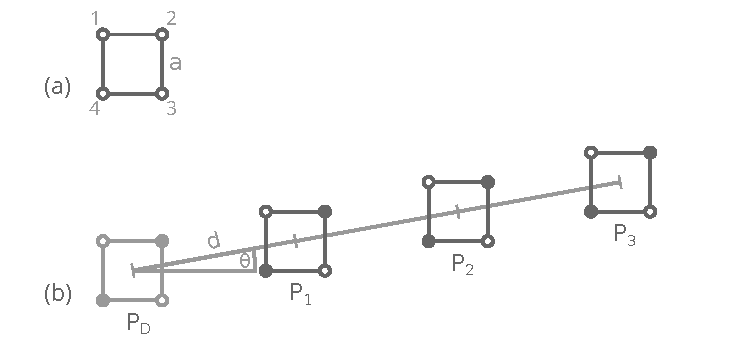
\includegraphics{short_wire}
  \caption
  [Parameterizing QCA layouts]
  {Parameterizing QCA layouts. (a) The edge length of a QCA cell is
  denoted by $a$. The dots of each cell are numbered clockwise. (b) A
  three-cell wire. The cell-cell distance is denoted by $d$, the cell-cell angle
  by $\theta$. The wire's input is set by the driver cell's polarization $P_D$,
  the active cells' polarizations are $P_1$, $P_2$, and $P_3$.}
  \label{fig:short_wire}
\end{figure}

To parameterize the Coulomb term $V_{kl}$ and specifically $r_{ij}$, the
distance between quantum dots $i$ and $j$, we introduce the cell edge length $a$
and the cell-cell distance $d$, as illustrated in
Fig.~\ref{fig:short_wire}(a)~and~(b), where we have used a short line of cells
as an example QCA system. The angle between adjacent cells is denoted by
$\theta$. Ideally each cell should be in logic state 0 or logic state 1, but,
of course, in practice a cell can be in any superposition of the two states or
even in a different state altogether. The \emph{cell polarization} $P_k$
quantifies the state of the cell,
\begin{equation}
  \label{eq:polarization}
  P_k = \frac{1}{2} \left( n_{4k+2} + n_{4k+4} - n_{4k-1} + n_{4k-3} \right) \, ,
\end{equation}
where the dots in each cell are numbered clockwise as indicated in the figure.
We have also introduced the shorthand notation $n_i = n_{i\uparrow} +
n_{i\downarrow}$. The cell polarization is $P_k = -1$ for a logic 0 and $P_k =
+1$ for a logic 1 state. Without any external input the polarization of a cell
will be $P_k = 0$. In the example line of cells, the input is set via the
driver cell's polarization $P_D$ at the left end. The driver cell's four static
point charges are adjusted to reflect the desired polarization $P_D$. For QCA,
the cell polarization really is the observable of utmost interest. It indicates
whether a cell is more in logic state 0 or logic state 1 and how polarized the
cell is, where ideally it should always be fully polarized, $|P_k| = 1$. In
short, the cell polarizations will indicate how well the QCA approach works for
a given system and, unsurprisingly, calculating cell polarizations for various
geometric layouts over a wide range of system parameters will be our main focus.

The QCA cell is characterized by three energy scales: the nearest-neighbour
hopping $t$, the nearest-neighbour Coulomb repulsion $V_1 = \frac{1}{a}$, and
the on-site Coulomb repulsion $U$. For QCA operation, $U$ is usually assumed to
be large enough that doubly occupied states are gapped out. We can introduce
$V_0 = \frac{1}{\sqrt{2} a}$, the energy scale for next-nearest-neighbour
Coulomb repulsion, which is realized when both electrons sit diagonally at
opposing corners of the cell---our preferred $P_k=\pm1$ states, ideally the
ground state. Conversely, $V_1$ corresponds to both electrons occupying the edge
of the cell. Again, for QCA operation we would like the edge states to be
sufficiently gapped out. In other words, the energy gap, 
\begin{equation}
  \label{eq:deltaV}
  \Delta V = V_1 - V_0 = \frac{2 - \sqrt{2}}{2} \frac{1}{a} \approx 0.3 V_1
\end{equation}
should be large compared to temperature $\Delta V \gg T$, and similarly $U \gg
\Delta V \gg T$. The competition between temperature $T$ and $V_1$ will thus
directly influence how polarized a cell is. In addition, $V_1$, which seeks to
order the cell, will compete with $t$, which delocalizes and disorders the
electrons. QCA is thought to function in a regime where Coulomb is the dominant
energy scale and hopping is a small perturbation: the ratio $V_1/t$ is large.
But it is also clear that if $V_1/t$ becomes too large, for example by taking $t
\rightarrow 0$, the system slows down and eventually freezes, which is rather
undesirable for QCA operation as well. In essence we can describe a cell by the
ratios $V_1/t$, $U/t$, and $T/t$. By similarly expressing the cell-cell distance
in units of the cell size $d/a$, we characterize any QCA system in dimensionless
units.


\section{Basic characterization}
\label{sec:basic_characterization}

\begin{figure}
  \center
  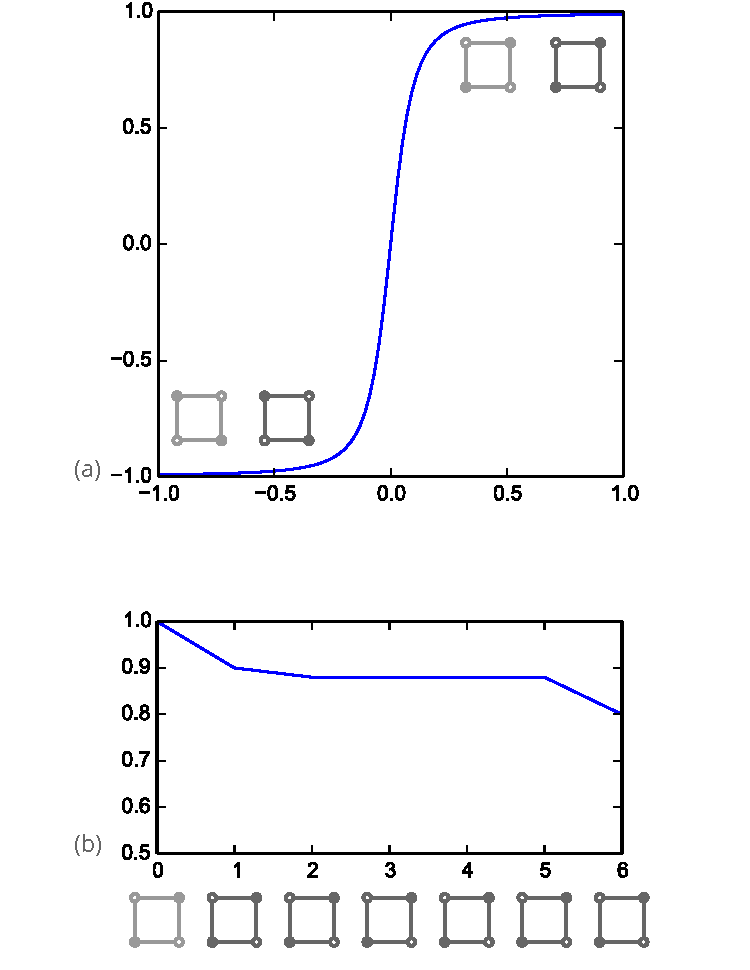
\includegraphics{qca_characterization}
  \caption
[Basic characteristics of QCA devices]
{
Basic characteristics of QCA devices, schematically. (a) The response of a
cell's polarization to a driver cell's polarization is non-linear and exhibits
gain. This gain has been used extensively to argue for the QCA approach's
inherent robustness. (b) Cell polarizations of a six-cell wire with input
polarization $P_D = 1$, as calculated with the intercellular Hatree
approximation. Most cells are polarized with the same saturation polarization
and only the leftmost and rightmost cells deviate slightly. In this picture, the
output polarization does therefore not depend on the wire length.
}
  \label{fig:qca_characterization}
\end{figure}

At the time of this writing, the QCA idea is over twenty years old. Naturally,
the fundamental building blocks of QCA circuitry such as the single cell itself,
the wire, and the majority gate have been characterized. Interestingly,
time-independent properties were investigated relatively briefly and arguably
not exhaustively. The bulk of the existing theoretical work soon came to focus
on system dynamics, the building of large-scale computing architectures with the
QCA paradigm, and specific potential experimental implementations. Previous work
on the characterization of time-independent QCA properties yielded two main
results. First, the cell-cell response, that is, how the polarization of one
cell responds to the polarization of a neighbouring cell, was established to be
non-linear and exhibit gain \cite{lent1993quantum}. Therefore, even an only
partially polarized cell would fully polarize the cell next to it,
Fig.~\ref{fig:qca_characterization}(a). Of course, gain is highly desirable,
if not essential, for building digital circuits. It compensates for any loss or
imperfections and makes the scheme overall robust. Not coincidentally, CMOS
technology is built around the MOSFET transistor with gain as one of its
intrinsic properties. Second, lines of cells were seen to be polarized with an
almost constant polarization throughout the whole line,
Fig.~\ref{fig:qca_characterization}(b) \cite{lent1993lines}: apart from a few
cells next to the driver cell, all remaining cells in the line would be
polarized with the same \emph{saturation polarization}. As a consequence, the
output polarization should not depend on the number of cells in the line. The
saturation polarization was observed to be largely independent of the driver
cell's polarization, but solely determined by the system's parameters such as
the hopping $t$ and the Coulomb energy $V_1$. For unfavourably chosen
parameters, the saturation polarization might be very small, but over a wide
range of system parameters it was shown to be close to perfect. For example, for
large hopping $t$, the saturation polarization is expected to be zero. If $t$ is
then decreased and passes a critical value $t_c$, a second-order phase
transition takes place. The saturation polarization becomes non-zero and in
fact very quickly close to perfect as $t$ is further decreased. In addition to
the cell-cell response and the analysis of a line of cells, larger QCA
structures such as the majority gate were reported to function correctly for a
select set of parameters but were not analyzed in depth. Overall, the physical
picture emerging from the early time-independent calculations is of bistable
cells readily snapping into the correct fully polarized state throughout the
whole device. It is a picture where the QCA approach works robustly and in fact
almost perfectly over a presumably wide range of parameters. It is the
prevailing picture to this day. It is also quite wrong.

These early calculations of time-independent QCA properties concentrated almost
exclusively on the ground state of the system (with one exception
\cite{tougaw1993bistable}). However, focusing solely on the ground state is not
sufficient. While the QCA approach is intended to be operated ``close to the
ground state,'' at least the first excited state is needed to obtain an estimate
for the operational temperature for these devices---a parameter of significant
practical interest. More subtly, what the QCA idea calls the ground state
actually corresponds to multiple states, namely one spin singlet and three spin
triplet states for $P=-1$ and $P=1$, respectively, in each cell. While these
states can reasonably be expected to be near-degenerate, a thorough study of QCA
should still consider them. In more practical terms, QCA is expected to operate
at finite temperatures, so simulating the devices at non-zero temperature is
appropriate. Similarly, the existing work on time-independent QCA properties is
not exhaustive with regard to the exploration of other parameters. For example,
while the saturation polarization's dependence on $V_1$ and $t$ is roughly
mapped out, concrete numerical values for these quantities are hard to come by.
In other cases, the Coulomb scale $V_1$ is not indicated explicitly at all.
Cells are assumed to be charge-neutral, but the effects of non-charge-neutrality
are not investigated.  Different cell-cell distances are not discussed, nor what
system parameters should be chosen for optimal performance.

The exact numerical simulation of QCA systems is challenging and in fact
intractable for all but the smallest structures. Therefore, approximations are
necessary. In the literature on QCA two approximations are prevalent: the
intercellular Hartree approximation (ICHA) and the two-states-per-cell
approximation \cite{lent1993quantum} \cite{tougaw1996dynamic}. Most of the
studies of time-independent QCA properties employ the ICHA. Only the cell-cell
response is calculated with a ``full'' quantum mechanical model, where the
``full'' model is actually already the reduced Hilbert space of exactly two
electrons per cell. ICHA is a mean field scheme: the Hamiltonian of one cell is
solved exactly in the mean field of the polarizations of all the other cells.
More specifically, the cell-cell interaction term $H^{cc}_{kl}$ in
equation~\eqref{eq:H_cell} is rewritten
\begin{equation}
\begin{split}
  \label{eq:H_kl_meanfield}
  H^{cc}_{kl} 
  %
  &=
  %
  \sum_{\substack{i \in k\\j \in l}} V_{ij} \left( n_i - q \right) \left( n_j - q \right) \\
  %
  &\approx
  %
  \sum_{\substack{i \in k\\j \in l}} V_{ij} 
       \left[ \left( n_i - q \right) \left( \left< n_j \right> - q \right)
              +
              \left( \left< n_i \right> - q \right) \left( n_j - q \right)
       \right] \, ,
\end{split}
\end{equation}
and, introducing the mean field for dot $i$ on cell $k$,
\begin{equation}
  \label{eq:V_meanfield}
  \tilde{V}_i^k
  = \sum_{l \ne k} \sum_{j \in l} \left( \left< n_j \right> - q \right)
  = \sum_{l \ne k} \mathcal{F} \left[ \left< P_l \right> \right] \, ,
\end{equation}
the one-cell mean field Hamiltonian becomes
\begin{equation}
  \label{eq:H_meanfield}
  H^{\mathrm{MF}}_k
  = H^c_k + \sum_{i \in k} \left( n_i - q \right) \tilde{V}_i^k \, .
\end{equation}
Because the cell polarization is directly related to the occupancies of the
sites of the cell, we have $\tilde{V}_i^k = \tilde{V}_i^k(\left<P_l\right>)$.
Solving the one-cell Hamiltonian allows one to compute the polarization $\left<
P_k \right>$ of the cell, which in turn is used to set the mean field
originating from all other cells. The procedure is repeated until a
self-consistent cell polarization and thus self-consistent solution for
Equation~\eqref{eq:H_meanfield} is found. By using $n_i n_j \approx n_i \left<
n_j \right> + \left< n_i \right> n_j$ mean field approximations neglect quantum
fluctuations. Only at high dimensionality can these fluctuations really tend to
zero, and indeed mean field schemes can be shown to become exact in the limit of
infinite dimensionality \cite{Fehske}. Conversely, for low dimensional systems
fluctuations are more important and mean field approximations are intuitively
expected not to work well. As an uncontrolled approximation, the validity of a
mean field approach has to be verified on a case by case basis.  Consequently,
because QCA is quasi-one-dimensional, it is arguably not well suited for a mean
field treatment. Even then a mean field approximation might be appropriate as a
first stab at the problem. But ICHA, having been introduced in the very first
QCA paper, was never properly verified or complemented by more accurate methods.
It is rather remarkable that a large part of the existing work on QCA
characterization rests, directly or indirectly, on an approximation that can
reasonably be expected to give wrong results. And indeed, in the context of the
dynamic properties of QCA, it has been known for a long time that ICHA does go
wrong \cite{toth2001role}. Much more recently, it has been shown very explicitly
that even for the single cell-cell response ICHA introduces artefacts that are
clearly non-physical \cite{taucer2012consequences}. As an intuitive simple
example where ICHA will give wrong results we can go back to the infinitely long
wire we already discussed above: we argued that due to entropy the infinite wire
can only be ordered at zero temperature. In contrast, a mean field approximation
will predict order up to a finite critical temperature. 
% TODO: correction from Kevin after "verified on a case by case basis":
% (especially in the case of discrete degrees of freedom where the Mermin Wagner
% theorem does not apply [ref])

For the calculation of time-dependent properties, the two-states-per-cell
approximation is typically used, precisely because it was realized that ICHA is
not sufficient, for example to calculate the switching behaviour of some
majority gate structures. Perplexingly, in the literature the two-state
approximation is motivated and justified by the ICHA picture
\cite{tougaw1996dynamic}. Starting from the observation that cells in a wire are
polarized with a saturation polarization $P_{\textrm{sat}}$---in ICHA
calculations---a cell is represented by two basis states, corresponding to $P =
P_{\textrm{sat}}$ and $P = - P_{\textrm{sat}}$. In a loose sense, the
two-states-per-cell model thus comes from a picture of how we would like QCA to
work: perfectly bistable, interacting cells.  The approximation has been
verified to the extent that it was shown that the ground state of the full
quantum mechanical model can be represented nearly perfectly by the two-state
basis, but only for one cell and for one particular set of system parameters. In
a more rigorous treatment it should be possible to clearly derive the two-state
model as the correct emerging low-energy Hamiltonian from the original extended
Hubbard model. Such a derivation would also reveal the parameter regime in which
the effective two-state Hamiltonian is valid. We will attempt the derivation in
due course. In contrast to the ICHA, the two-states-per-cell approximation
retains inter-cell entanglement and therefore yields more correct results, not
only for dynamics, but also for time-independent properties. This comes at the
cost of exponential scaling for the two-state model, whereas ICHA scales
linearly in system size. Therefore, even with the two-state approximation only
relatively small QCA devices are computationally feasible. As a final note, the
two-state model is clearly a close cousin to the transverse field quantum Ising
model, where the two polarization states correspond to a pseudo spin and the
hopping is like a transverse field, flipping cell polarizations.


\section{Exact diagonalization}

We use the numerical method of exact diagonalization \cite{Fehske} to simulate
QCA systems described by the Hamiltonian \eqref{eq:H_QCA}. In principle, exact
diagonalization is a straightforward method: for a chosen basis the matrix of
the Hamiltonian is constructed explicitly and then diagonalized, yielding the
eigenenergies and eigenstates of the system. With that we know everything about
the system and can calculate observables of interest. The problem is that memory
consumption scales as $N_s^2$ and the computational cost roughly as $N_s^3$,
where $N_s$ is the size of the state space; and the number of states scales
exponentially with system size, $N_s = 4^{N_d} = 256^{N_c}$. $N_d$ denotes the
number of dots and $N_c$ the number of cells. As an example, to store the full
Hamiltonian matrix of a two-cell QCA system requires 3GB of memory, and to store
the Hamiltonian matrix of a three-cell system already requires 2000TB. That's
clearly not feasible on any available computer. As a side note, we cannot employ
projective algorithms such as Lanczos \cite{Fehske}, because we are interested
in finite temperatures and therefore need the full energy spectrum. Typically,
projective schemes are only useful to calculate the ground state or the few
lowest energy states. 

%
To decrease the memory requirements and computational cost of
exact diagonalization, symmetries must be exploited. The Hamiltonian matrix is
actually quite sparse---most entries are zero. By using symmetries and a
suitable basis, the Hamiltonian matrix can be brought into block diagonal form
and then only those much smaller blocks need to be diagonalized. Our QCA system
is symmetric with respect to the total particle number $\hat{N} = \sum_i
\hat{n}_{i\uparrow} + \hat{n}_{i\downarrow}$ and the total spin $\hat{S} =
\sum_i \hat{n}_{i\uparrow} - \hat{n}_{i\downarrow}$, i.e.\ $[\hat{N},\hat{H}]_-
= [\hat{S},\hat{H}]_- = 0$. If we now use basis states which are eigenstates of
the symmetry operators, $\ket{n,s,l}$, with
%
\begin{equation}
\begin{split}
  \hat{N} \ket{n,s,l} &= n \ket{n,s,l} \, , \\
  \hat{S} \ket{n,s,l} &= s \ket{n,s,l} \, ,
\end{split}
\end{equation}
%
then we have
%
\begin{equation}
\begin{split}
  \bra{n^{\prime},s^{\prime},l^{\prime}} [\hat{N},\hat{H}]_- \ket{n,s,l} = 
  (n^{\prime} - n) \bra{n^{\prime},s^{\prime},l^{\prime}} \hat{H} \ket{n,s,l}
  \stackrel{!}{=} 0 \\
  \bra{n^{\prime},s^{\prime},l^{\prime}} [\hat{S},\hat{H}]_- \ket{n,s,l} = 
  (s^{\prime} - s) \bra{n^{\prime},s^{\prime},l^{\prime}} \hat{H} \ket{n,s,l}
  \stackrel{!}{=} 0
\end{split}
\end{equation}
%
and therefore
%
\begin{equation}
  \bra{n^{\prime},s^{\prime},l^{\prime}} \hat{H} \ket{n,s,l} = 0 \qquad
  \textrm{for } n \ne n^{\prime} \textrm{ or } s \ne s^{\prime} \, .
\end{equation}
%
Consequently, in ordering basis states by the symmetry operators' eigenvalues,
the Hamiltonian matrix becomes block diagonal, where the blocks are labelled by
$n$ and $s$. The blocks can be constructed and diagonalized separately, and all
observables can then be calculated block-wise as well, hence vastly reducing
memory requirements and computational time. In our implementation, however, we
do keep all blocks in memory simultaneously. This still yields considerably
reduced memory usage and the same speedup in computational time. For the QCA system
the single largest block is the spin zero sector at half-filling. Its size is
%
\begin{equation}
  N_s^{\prime} = \binom{N_d}{\frac{1}{2} N_d}^2 \, .
\end{equation}
%
This corresponds to memory requirements of 180MB for two cells and 5400GB for
three cells. Thus, although this is a considerable improvement for the two-cell
system (not least in computational time), the three-cell system still remains
unreachable with conventional computer hardware. To access larger systems we
need to introduce approximations, which we will pursue in detail and with great
care in the following chapter.

Computational physics is, true to its name, to considerable extent concerned
with writing computer code. If ingenious algorithms which bring sophisticated
physical problems to the computer are the art that excites the computational
physicist's intellect, then writing good computer code is the craft. It is a
curious fact that traditionally in computational condensed matter physics,
little weight has been put on collaboration on the code level, the development
of common tools, coding techniques, and the code itself. This not only
frustrates the newcomer to the field, for it is a long way from a formally
stated algorithm to a correct and efficient implementation, but also poses a
more fundamental problem to science in a time when computing has long become an
essential part of it. Scientific results obtained from sophisticated numerical
algorithms can be difficult to verify and reproduce without an openly available
implementation of those algorithms. But verification and reproducibility are
core assets of the scientific process. Fortunately, the culture is slowly
changing. In computational condensed matter physics, the ALPS and Abinit
projects provide open implementations of a variety of commonly used methods and
algorithms \cite{bauer2011alps} \cite{gonze2009abinit}. In the wider scientific
community, IPython is a shining example of building a powerful computational
tool collaboratively, with a huge impact across disciplines
\cite{perez2007ipython}.

Our QCA exact diagonalization implementation is written in C++ and uses the
excellent Eigen linear algebra library \cite{eigen}. Matrices are stored in
sparse representation, except for the block-wise diagonalization itself,
performed by Eigen, where we use dense matrices. The basis states can be
filtered and sorted, for example to truncate the Hilbert space to a specific
charge sector and to exploit symmetries. We do not build the Hamiltonian matrix
directly, but instead construct creation and annihilation operator matrices.
Therefore, operators such as the Hamiltonian and the polarization can be
expressed in an intuitive, almost mathematical notation. We employ the
``curiously recurring template'' pattern to achieve simple static polymorphism,
avoiding the overhead of runtime polymorphism \cite{andrei2001modern}. In less
abstract terms, this allows us to reuse code, for example the Hamiltonian, for
the conceptually similar, but physically quite different various QCA models
which we are going to introduce in detail in the next chapter. Our C++ code
cannot be executed directly, but is instead compiled as an extension module for
the Python language, via the Boost library's Boost.Python \cite{boost}. We also
use the unit testing framework from the Boost library. In our experience, making
the C++ code available in Python provides enormous benefits. With Python data
input, output and storage becomes a breeze, especially compared to the chore
these tasks are in pure C++. Python makes it easy to script and distribute
(i.e.\ simply parallelize) simulation runs, and, being well established in the
scientific community, comes with extensive libraries for data analysis and
plotting, for example SciPy and Matplotlib \cite{scipy}
\cite{hunter2007matplotlib}. Consequently, the integration with Python
facilitates quickly trying out new ideas, implementing new features and more
fluid data analysis. The advent of the fantastic IPython notebook ties all of
these pieces together in a consistent, productive and highly enjoyable workflow
\cite{perez2007ipython}. The IPython notebook is also an apt format for
effectively communicating results with colleagues. The disadvantages of the
Python integration are the additional dependencies, although both Python and
Boost are commonly available on any number of platforms these days, and the more
involved (and hence error-prone) build process. We have written a small Python
library to support our data storage and organization needs. The library
facilitates storing and retrieving data in standard file formats and allows to
define and run ``numerical experiments,'' which can be distributed across
multiple computers. Both the QCA exact diagonalization code and the Python
library are available under an open license on GitHub \cite{githubqca}
\cite{githubcoma}.

\chapter{Approximations}
\graphicspath{{../gfx/chapter02/}{../plots/chapter02/}}


\section{Fixed charge model}

Exact diagonalization scales exponentially with system size. With the full
\emph{grand canonical} QCA Hamiltonian \eqref{eq:H_QCA} only devices of up to
two cells are computationally feasible. Therefore, we need to introduce
approximations to access larger systems. Approximating means to simplify.
However, by carefully establishing successive approximations and their limits,
we also reduce the problem to its essential ingredients and thus, hopefully, we
gain a better understanding of the QCA approach. As a first step, we reduce the
Hilbert space to states with a fixed number of particles per cell. We disallow
any charge fluctuations, both for the system as a whole and for each individual
cell. With that, we omit the chemical potential term in the Hamiltonian, $\mu =
0$, and prohibit inter-cell hopping. This is a major simplification. However, it
is in line with the QCA idea: the approach requires a fixed number of charges
per cell, typically two electrons, and cells are thought to interact only via
Coulomb forces. If the \emph{fixed charge} approximation is not valid for a
given system, then there is no hope of implementing QCA on it. For experimental
systems like the atomic silicon quantum dots, it should always be possible, at
least in principle, to tune the system parameters so that for a given cell
layout each cell is occupied by the same number of electrons. The
two-electrons-per-cell sector has to be lowest in energy and other particle
number sectors need to be sufficiently gapped out, that is, at an energy much
larger than temperature. Of course, in practice there are very clear limits as
to how much the system parameters can be tuned. Any QCA cell layout considered
within the fixed charge approximation cannot necessarily be readily implemented
on a given real-world material system.

For the fixed charge model, the state space scales as $N_s = \binom{8}{2}^{N_c}
= 28^{N_c}$ ($N_c$ is the number of cells). Using symmetries, the largest block
of the Hamiltonian matrix is the spin zero sector, of size $N_s^{\prime} =
16^{N_c}$. On conventional computer hardware, systems of up to four cells are
possible, with memory requirements of 32GB. However, such calculations take very
long and therefore three-cell systems are the practical limit.


\section{Bond model}

%
\begin{figure}
  \center
  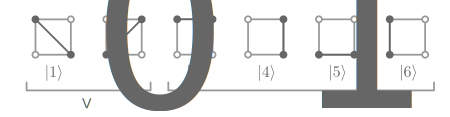
\includegraphics{bond}
  \caption{
  The six bonds of a QCA cell. The basis of a QCA cell in the fixed charge
  picture consists of six bonds and four doubly occupied dots. Each bond
  corresponds to one spin singlet and three spin triplet states. The bond model
  neglects doubly occupied states and keeps only one state per bond for a total
  of six states per cell. From those, the Ising approximation only retains
  the two lowest energy states, $\ket{1}$ and $\ket{2}$ with energy $V_0$.
  }
  \label{fig:bond}
\end{figure}
%
At its heart, QCA is a semi-classical idea. It relies dominantly on
charge-charge interactions and ignores the particle spin. Therefore, as a next
step in our quest to access larger system sizes, we neglect the spin degrees of
freedom. The 28 states of each cell in the fixed charge model can be reorganized
into four doubly occupied dots and six bonds, illustrated in
Fig.~\ref{fig:bond}. Each bond corresponds to one spin singlet and three spin
triplet states. The \emph{bond} approximation only keeps one state for each bond
and discards the doubly occupied states as well. With the bond model we thus
assume that singlet and triplet states are qualitatively and energetically
equivalent, and that doubly occupied dots are sufficiently gapped out, that is,
$U \gg T$. Because QCA ignores the spin, singlets and triplets should be
qualitatively the same---for example, they should yield the same cell
polarizations. However, we can speculate that virtual double-occupancy lowers
the energies of the singlet states and therefore introduces a small
singlet-triplet splitting. Neglecting this small splitting presumably does not
introduce a large error, but we will have to verify this assumption and look at
the splitting in more detail in due course. For the bond model the QCA
Hamiltonian reduces to
%
\begin{equation}
  \label{eq:H_bond}
  H = - \sum_{\left<ij\right>} t c_i^{\dagger} c_j
      + \sum_{i<j} V_{ij} \left( n_i - q \right) \left( n_j - q \right) \, .
\end{equation}
%
With six bond states per cell, the Hilbert space of the bond model is $N_s =
6^{N_c}$ ($N_c$ the number of cells). Five and six cells are doable, with memory
requirements of 460MB and 16GB, respectively, but for practical calculations
five-cell systems really are the limit. For the bond model there are no
symmetries that can be exploited.


\section{Ising model}

%
\begin{figure}
  \center
  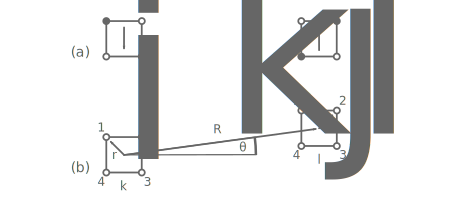
\includegraphics{ising}
  \caption{
  (a) The Ising approximation identifies each cell with a pseudo spin. Logic 0
  corresponds to spin down and logic 1 to spin up. (b) QCA cells $k$ and $l$. 
  }
  \label{fig:ising}
\end{figure}
%
A linear array of QCA cells where each cell has a state of logic 0 or 1 is
reminiscent of a 1D spin $\frac{1}{2}$ chain. Indeed, if we reduce the basis to
only two states per cell, down from six states in the bond picture, we can map
the QCA system to a transverse-field Ising model with long-ranged interactions.
This is an attractive proposition: The smaller Hilbert space allows for larger
system sizes with our exact diagonalization method; more importantly, the
transverse-field Ising model is amenable to sign-problem-free Stochastic series
expansion (SSE) quantum Monte Carlo schemes \cite{Sandvik2003}. These methods do
not scale exponentially\footnote{SSE quantum Monte Carlo methods roughly scale
as $N \ln N$ where $N$ is the system size.} and consequently allow access to
much larger systems. Last, but not least, such a mapping connects the QCA
approach to the established and well studied Ising model. The prospect hinges on
the assumption that the two-states-per-cell basis actually is a good
approximation for QCA systems. And while bistable two-state cells are certainly
the picture we have in mind when we talk about QCA, it is not \emph{a priori}
clear whether this is a correct physical picture. The transverse-field Ising
model is equivalent to the two-states-per-cell approximation that has been used
extensively, but was never satisfyingly derived, in the literature to study the
dynamics of QCA systems.

We use the bond Hamiltonian \eqref{eq:H_bond} as the starting point. We
had already discussed in the last chapter that such a Hamiltonian can be
decomposed into single-cell terms and cell-cell interaction terms,
\begin{equation}
  H = \sum_k H^c_k + \sum_{k<l} H^{cc}_{kl} \, .
\end{equation}
In comparison, the transverse-field Ising model is described by
%
\begin{equation}
  \tilde{H} = - \sum_k \gamma S^x_k + \sum_{k<l} J_{kl} S^z_k S^z_l \, .
\end{equation}
%
Thus, we would like to map the single cell term $H^c_k$ to the transverse-field
term $-\gamma S^x_k$ and the Coulombic cell-cell interaction $H^{cc}_{kl}$ to
the Ising term $J_{kl} S^z_k S^z_l$. Each cell $k$ is identified with a pseudo
spin $S^z_k$, specifically logic 0 with spin down and logic 1 with spin up, as
illustrated in Fig.~\ref{fig:ising}(a). We will first look at how the QCA cell
can be represented by only two basis states and derive an approximate expression
for the transverse field $\gamma$. Then we will use a multipole expansion to
derive $J_{kl}$ from the cell-cell Coulomb interaction.

To arrive at a single-cell-basis with only two states we can, in principle,
follow a similar prescription as for the fixed charge and bond approximations:
we neglect high-energy states which are assumed to be gapped out. In this case,
the neglected states are the four edge states with Coulomb energy $V_1$,
$\ket{\psi_Q} = \left\{ \ket{3}, \ket{4}, \ket{5}, \ket{6} \right\}$,
illustrated in Fig.~\ref{fig:bond}, where we have introduced $\ket{\psi_Q}$ to
denote the high-energy subspace of the single-cell Hilbert space. We only keep
the low-energy diagonal states $\ket{\psi_P} = \left\{ \ket{1}, \ket{2}
\right\}$ with Coulomb energy $V_0$. Of course, these two states are exactly our
logic 0 and logic 1 state, or, in the Ising language, $\ket{\downarrow} \doteq
\ket{1}$ and $\ket{\uparrow} \doteq \ket{2}$. Here, $\ket{\psi_P}$ denotes the
low-energy subspace. For the high-energy states to be sufficiently gapped out,
we require $\Delta V = V_1 - V_0 \gg T$. In contrast to the fixed charge and
bond model, merely truncating the Hilbert space is not sufficient for the Ising
model. For our previous two approximations, the Hamiltonian had remained
essentially unchanged, apart from dropping no longer relevant terms, such as the
chemical potential term or the Hubbard $U$ term. The retained states were
exactly the same states as in the full, untruncated model. But with only two
states per cell the existing Hamiltonian \eqref{eq:H_bond} does not ``work'':
There is no process that takes the cell from $\ket{1}$ to $\ket{2}$ and the
system would be stuck in either of the two spin states eternally. In the bond
picture, in comparison, for the system to transition from state $\ket{1}$ to
$\ket{2}$ it can take different paths, for example $\ket{1} \rightarrow \ket{3}
\rightarrow \ket{2}$, consisting of two hopping processes with an interim
high-energy edge state. We need to derive an effective, low-energy Hamiltonian
from the bond model that treats those processes perturbatively, as
\emph{virtual} excitations, yielding an effective hopping term for the
transition $\ket{1} \leftrightarrow \ket{2}$. This effective hopping is
precisely the transverse field $\gamma$ which flips the spin in the Ising
picture.
% TODO: $-\gamma S^x_k = -\gamma \frac{1}{2} \left( S^+_k + S^-_k \right)$.

A single QCA cell is described by the time-independent Schr\"odinger equation
$H^c_k \ket{\psi} = E_k \ket{\psi}$, with $\ket{\psi} = \left[ \ket{\psi_P}
\ket{\psi_Q} \right]$. Our aim it to truncate the basis to $\ket{\psi_P}$ and
derive an effective Hamiltonian $\tilde{H}^c_k$ with the subspace
Schr\"odinger equation $\tilde{H}^c_k \ket{\psi_p} = E_k \ket{\psi_p}$. Using
the basis depicted in Fig.~\ref{fig:bond}, the single-cell bond Hamiltonian is
very simple and can be written down explicitly. As the single-cell Hamiltonian
is the same for all cells, we can drop the index $k$.
%
\begin{equation}
\begin{split}
  \label{eq:H_marix}
  H^c
  &=
  %
  \left(
  \begin{array}{cc|cccc}
    V_0 & 0   & -t  & -t  & -t  & -t  \\
    0   & V_0 & -t  & -t  & -t  & -t  \\
    \hline
    -t  & -t  & V_1 & 0   & 0   & 0   \\
    -t  & -t  & 0   & V_1 & 0   & 0   \\
    -t  & -t  & 0   & 0   & V_1 & 0   \\
    -t  & -t  & 0   & 0   & 0   & V_1 \\
  \end{array}
  \right) \\[1em]
  %
  &=
  \left(
  \begin{array}{cc}
    H_{PP} & H_{PQ} \\
    H_{QP} & H_{QQ} \\
  \end{array}
  \right)
\end{split}
\end{equation}
%
Here, we have partitioned the Hamiltonian into four blocks, $H_{PP}$, $H_{QQ}$,
$H_{PQ}$, and $H_{QP}$, corresponding to the low-energy subspace $\ket{\psi_P}$,
the high-energy subspace $\ket{\psi_Q}$, and transitioning between the subspaces.
With this partitioned Hamiltonian the time-independent Schr\"odinger equation is
%
\begin{equation}
  \label{eq:SE}
  %
  \begin{pmatrix}
    H_{PP} & H_{PQ} \\
    H_{QP} & H_{QQ} \\
  \end{pmatrix}
  \begin{pmatrix}
    \psi_P \\
    \psi_Q \\
  \end{pmatrix}
  =
  E
  \begin{pmatrix}
    \psi_P \\
    \psi_Q \\
  \end{pmatrix}
  \, .
  %
\end{equation}
%
Writing out the matrix equation as two equations explicitly, and eliminating
$\ket{\psi_Q}$ yields 
%
\begin{equation}
  H_{PP} \ket{\psi_P} + H_{PQ} \frac{1}{E - H_{QQ}} H_{QP} \ket{\psi_P}
  =
  E \ket{\psi_P}
\end{equation}
%
and therefore
%
\begin{equation}
  \label{eq:H_effective}
  \tilde{H}^c = H_{PP} + H_{PQ} \frac{1}{E - H_{QQ}} H_{QP} \, .
\end{equation}
%
Assuming that the system is predominantly in the subspace spanned by
$\ket{\psi_P}$ and additionally that the hopping is very small, $t \ll V_0$, we
can approximate $E \approx V_0$. We write out the matrix multiplications and use
$\left( H_{PP} \right)_{ij} = \left( V_0 \right)_{ii} \delta_{ij}$, $\left(
H_{PQ} \right)_{ij} = \left( -t \right)_{ij}$, and so on. The effective
Hamiltonian becomes
%
\begin{equation}
\begin{split}
  \tilde{H}^c_{ij}
  %
  &=
  \left( V_0 \right)_{ii} \delta_{ij}
  + \left( - t \right)_{ik}
    \left( V_0 - V_1 \right)^{-1}_{kk}
    \left( - t \right)_{kj} \\
  %
  &=
  \left( V_0 \right)_{ii} \delta_{ij}
  - \left( \frac{4 t^2}{\Delta V} \right)_{ij} \, .
\end{split}
\end{equation}
%
As the system remains unchanged upon adding a constant term to the Hamiltonian,
we can subtract the constant diagonal term $\tilde{H}_{ii} = V_0 - \frac{4
t^2}{\Delta V}$, and arrive at
%
\begin{equation}
  \tilde{H}^c
  =
  \begin{pmatrix}
    0 & - \frac{4 t^2}{\Delta V} \\
    - \frac{4 t^2}{\Delta V} & 0 \\
  \end{pmatrix} \, .
\end{equation}
%
The off-diagonal matrix elements are the effective hopping, transitioning the
system between its two states $\ket{1} \leftrightarrow \ket{2}$. If we now
compare this matrix with the transverse-field term of the Ising model,
%
\begin{equation}
\begin{split}
  \tilde{H}^c
  &=
  - \gamma S^x_k \\
  &=
  - \frac{1}{2} \gamma \left( S^+_k + S^-_k \right) \\[0.5em]
  &= 
  \begin{pmatrix}
    0 & - \frac{1}{2} \gamma \\
    - \frac{1}{2} \gamma & 0 \\
  \end{pmatrix} \, ,
\end{split}
\end{equation}
%
we identify the effective hopping as the transverse field $\gamma$,
%
\begin{equation}
  \label{eq:gamma}
  \gamma = \frac{8 t^2}{\Delta V} \, .
\end{equation}
%
The effective hopping is a virtual process involving two hopping processes in
the original bond model, yielding the $t^2$ in the numerator, and an interim
high-energy state gapped out by $\Delta V$, hence the $\Delta V$ in the
denominator. To arrive at the expression for the effective hopping $\gamma$ we
used the assumptions $\Delta V \gg T$ and $t \ll \Delta V$. As a reminder,
$\Delta V = V_1 - V_0 = \frac{2 - \sqrt{2}}{2} \frac{1}{a} \approx 0.3 V_1$.
Notably, the energy gap is independent of the compensation charge $q$. As the
derivation used only a single cell, it is also implicitely assumed that the
perturbations from other cells in the system are small, at least as far as the
effective hopping is concerned. If the hopping depended on the state of nearby
cells, then the effective Hamiltonian would be much more involved and certainly
could not be mapped to an Ising-like model.

We have successfully derived an effective hopping term and therefore also an
effective two-state model for the QCA Hamiltonian. With only two states per cell
the Hilbert space scales as $N_s = 2^{N_c}$ ($N_c$ the number of cells) and up
to 14 cells are computationally feasible, with memory requirements of 2GB. In
practice, we restrict the calculations to a maximum of 12 cells. For our
calculations, we can use the two-state approximation with the effective hopping
term, but still retain the original cell-cell interaction term $H^{cc}_{kl}$.
From a computational point of view, nothing is gained by expressing the
cell-cell interaction as an Ising interaction. However, deriving $J_{kl}$ from
$H^{cc}_{kl}$ is very rewarding conceptually and will already allow some key
insights into the characteristics of QCA devices. Therefore, we now undertake
the derivation of an expression for $J_{kl}$. The obvious starting point is the
cell-cell interaction term $H^{cc}_{kl}$, 
%
\begin{equation}
\begin{split}
  H^{cc}_{kl} 
  %
  &=
  %
  \sum_{\substack{i \in k\\j \in l}} V_{ij} \left( n_i - q \right) \left( n_j - q \right) \\
  %
  H^{cc}_{kl}
  %
  &= 
  %
  \sum_{\substack{i \in k\\j \in l}}
  \frac{ \left( n_i - q \right) \left( n_j - q \right) }
       { \left| \bm{R}_{kl} + \bm{r}_j - \bm{r}_i \right| } \\
  %
  &=
  \sum_{\substack{i \in k\\j \in l}}
  \frac{n_i n_j - q (n_i + n_j)}
       {\left| \bm{R}_{kl} + \bm{r}_{ij} \right|} \, ,
\end{split}
\end{equation}
%
where $i$ and $j$ sum over the four dots $1\ldots4$ of cell $k$ and $l$,
respectively, and $\bm{R}_{kl}$ denotes the vector between the centres of the cells,
see Fig.~\ref{fig:ising}(b). We have introduced $\bm{r}_{ij} = \bm{r}_j -
\bm{r}_i$ and dropped the constant $q^2$ term. There are only four possible
configurations for two interacting cells: $\uparrow\uparrow$,
$\downarrow\downarrow$, $\uparrow\downarrow$, and $\downarrow\uparrow$. Using
the shorthand notations $V_{ij} = \frac{1}{\left| \bm{R}_{kl} + r_{ij} \right|}
+ \frac{1}{\left| \bm{R}_{kl} - r_{ij} \right|}$ and $V_{00} = \frac{1}{\left|
\bm{R}_{kl} \right|}$, we calculate their energies explicitly.
\begin{align}
  %
  E^{\uparrow\uparrow}
  &=
  \left( 1 - 2 q \right) \left( 2 V_{00} + V_{24} \right)
  - q \left( 2 V_{12} + 2 V_{14} \right)
  \\
  %
  E^{\downarrow\downarrow}
  &=
  \left( 1 - 2 q \right) \left( 2 V_{00} + V_{13} \right)
  - q \left( 2 V_{12} + 2 V_{14} \right)
  \\
  %
  E^{\uparrow\downarrow}
  &=
  \left( 1 - 2 q \right) \left( V_{12} + V_{14} \right)
  - q \left( 4 V_{00} + V_{13} + V_{24} \right)
  \\
  %
  E^{\downarrow\uparrow}
  &=
  \left( 1 - 2 q \right) \left( V_{12} + V_{14} \right)
  - q \left( 4 V_{00} + V_{13} + V_{24} \right)
\end{align}
Note that the expression for two spin-down cells can be obtained from the
expression for two spin-up cells (and similarly $E^{\uparrow\downarrow}$ from
$E^{\downarrow\uparrow}$) simply by rotating the system by $90^{\circ}$, or
equivalently, by permuting the dot numbering: $1,2,3,4 \rightarrow 4,1,2,3$.
Symmetries can be exploited, for example $V_{43} = V_{12}$. Evidently,
$E^{\uparrow\downarrow} = E^{\downarrow\uparrow}$, which, given the highly
symmetric geometry of those cell arrangements, does not come as a surprise. But
crucially, we find $E^{\uparrow\uparrow} \ne E^{\downarrow\downarrow}$.
Therefore, we have a system with three distinct energy levels which we cannot
hope to represent with the solely two-level Ising term $J_{kl} S^z_l S^z_l$.
Instead, let us try to map to a \emph{modified} Ising model with a three-level
cell-cell interaction term of the form
%
\begin{equation}
  \label{eq:Ising_term}
  %
  \tilde{H}^{cc}_{kl}
  = 
  J_{kl} S^z_k S^z_l + 
  J^{\prime}_{kl} \left( S^z_k + S^z_l \right) \, .
\end{equation}
%
For this Hamiltonian we have the energies
%
\begin{align}
  \tilde{E}^{\uparrow\uparrow} - \tilde{E}^{\uparrow\downarrow}
  &=
  2J_{kl} + 2J^{\prime}_{kl} \\
  %
  \tilde{E}^{\downarrow\downarrow} - \tilde{E}^{\uparrow\downarrow}
  &=
  2J_{kl} - 2J^{\prime}_{kl}
\end{align}
%
which yields
%
\begin{align}
  \label{eq:Js_from_Es}
  J_{kl}
  &=
  \frac{1}{4} 
  \left( 
    \tilde{E}^{\uparrow\uparrow} + \tilde{E}^{\downarrow\downarrow}
    - 2 \tilde{E}^{\uparrow\downarrow} 
  \right) \\
  %
  J^{\prime}_{kl}
  &=
  \frac{1}{4}
  \left( \tilde{E}^{\uparrow\uparrow} - \tilde{E}^{\downarrow\downarrow} \right) \, ,
\end{align}
%
and therefore, identifying $E^{\uparrow\uparrow} = \tilde{E}^{\uparrow\uparrow},
E^{\downarrow\downarrow} = \tilde{E}^{\downarrow\downarrow}$, and so on,
\begin{align}
  \label{eq:J}
  %
  J_{kl}
  &=
  \frac{1}{4} 
  \left(
    4 V_{00} + V_{13} + V_{24} - 2 V_{12} - 2 V_{14}
  \right) \\
  %
  \label{eq:Jprime}
  %
  J^{\prime}_{kl}
  &=
  \frac{1}{4}
  \left( 1 - 2 q \right)
  \left( V_{24} - V_{13} \right) \, .
\end{align}
These results, while abstract, are remarkable in two ways. First, the newly
introduced term $J^{\prime}_{kl}$ vanished for $q=\frac{1}{2}$. In this case,
$E^{\uparrow\uparrow} = E^{\downarrow\downarrow}$. Thus, for charge neutral
cells we recover the genuine, unmodified transverse-field Ising model. Second,
the Ising $J_{kl}$ itself is independent of the compensation charge $q$. We
will see that $J_{kl}$ is the quadrupole-quadrupole cell-cell interaction, to
leading order. Thus, it is fair to say that $J_{kl}$ is the pure QCA
interaction. With the above equations we can also already look at rotational
symmetries of $J_{kl}$ and $J^{\prime}_{kl}$: $J_{kl}$ is invariant under
rotations by $90^{\circ}$ as can be seen by permuting the dots $1,2,3,4
\rightarrow 4,1,2,3$. This is what we expect intuitively. For example, a
horizontal straight line of cells ($\theta = 0^{\circ}$) should behave exactly
the same as a vertical straight line of cells ($\theta = 90^{\circ}$). In
contrast, $J^{\prime}_{kl}$ is not invariant under rotations by $90^{\circ}$. In
fact, applying the same dot permutation yields $J^{\prime}_{kl}
\xrightarrow{\,\, 90^{\circ}} - J^{\prime}_{kl}$. Consequently,
$J^{\prime}_{kl}$ is symmetric under rotations by $180^{\circ}$. It is also
clear that a non-zero $J^{\prime}_{kl}$ breaks the system's symmetry under spin
rotation---$\tilde{H}^{cc}_{kl}$ is not unchanged for $\uparrow\uparrow \,
\rightarrow \, \downarrow\downarrow$. This has profound implications for QCA.
For non-zero $J^{\prime}_{kl}$ we would, for example, expect different
polarization responses for two spin-down cells versus two spin-up cells, and as
a consequence the device would behave differently for logic 0 and logic 1
signals. From an application point of view, this is definitely not what we want.
For QCA operation we therefore require charge neutral cells and a genuine,
unmodified Ising model.

To obtain more tangible expressions for $J_{kl}$ and $J^{\prime}_{kl}$ we do a
multipole expansion of the $V_{ij}$ terms. Specifically,
%
\begin{equation}
\begin{split}
  \frac{1}{\left| \bm{R}_{kl} \pm r_{ij} \right|}
  &=
  \frac{1}{R_{kl}}
  \left( 
  1 \pm 2 \frac{\bm{r}_{ij} \hat{\bm{R}}_{kl}}{R_{kl}} + \frac{r_{ij}^2}{R_{kl}^2}
  \right)^{-1/2} \\
  &=
  \frac{1}{R_{kl}} \left( 1 \pm x + y \right)^{-1/2}
\end{split}
\end{equation}
%
is Taylor-expanded in $x$ and $y$, keeping all terms up to
$\mathcal{O}\left(\frac{a^4}{R_{kl}^5}\right)$, which corresponds to
quadrupole-quadrupole interactions. Plugging the results of the expansion back
into Eqs.~\eqref{eq:J} and \eqref{eq:Jprime} yields
%
\begin{align}
  \label{eq:J_}
  %
  J_{kl}
  &=
  \frac{ 1 }{ 32 }
  \left(
    9 - 105 \cos{4 \theta}
  \right)
  \frac{ a^4 }{ R_{kl}^5 }
  \\
  %
  \label{eq:Jprime_}
  %
  J^{\prime}_{kl}
  &=
  \left( 1 - 2 q \right)
  \left(
    \frac{ 3 }{ 2 } \sin{2 \theta} \frac{ a^2 }{ R_{kl}^3 } +
    \frac{ 5 }{ 4 } \sin{2 \theta} \frac{ a^4 }{ R_{kl}^5 }
  \right) \, .
  %
\end{align}
%
The leading order term of $J_{kl}$ is $R^{-5}$, the quadrupole-quadrupole
interaction. In contrast, the leading order term of $J^{\prime}_{kl}$ is
$R^{-3}$ and therefore, in general, $J^{\prime}_{kl}$ would be the dominating
term---yet another argument why a non-zero $J^{\prime}_{kl}$ is highly
undesirable for functioning QCA devices. Of course, we find our general symmetry
observations confirmed by these more concrete expressions for $J_{kl}$ and
$J^{\prime}_{kl}$: the former is invariant under $90^{\circ}$ rotations, the
latter only under rotations of $180^{\circ}$. Both terms vanish at select
angles. For example, we have $J^{\prime}_{kl} = 0$ for $\theta = 0^{\circ}$, so
that at least for an exactly straight line of cells we recover the unmodified
Ising model, even for non-charge-neutral cells. This does not help when building
more complex devices than a wire, of course, but might still be useful for some
experiments. As another example, $J_{kl} = 0$ for $\theta = 22.5^{\circ}$.
Conceivably, this could be exploited for device applications, to decouple
closely spaced cells. As multipole expansions, the obtained expressions for
$J_{kl}$ and $J^{\prime}_{kl}$ should be valid for large cell-cell distances. In
principle, an arbitrary number of higher order terms can be included to make the
expressions as exact as desired. In practice on the computer, however, we do not
use the multipole expansion at all, but simply sum up all Coulomb interactions
exactly. We will see in due course that for the small cell-cell distances that
we are typically interested in, an expansion up to $R^{-5}$ is indeed not
sufficient, and higher order terms would have to be included.

In summary, we have successfully mapped the QCA bond
Hamiltonian \eqref{eq:H_bond} to a modified transverse-field Ising model,
\begin{equation}
  \label{eq:H_Ising}
  %
  \tilde{H}
  =
  - \sum_k \gamma S^x_k
  + \sum_{k<l}
    \left[
      J_{kl} S^z_k S^z_l + 
      J^{\prime}_{kl} \left( S^z_k + S^z_l \right)
    \right] \, ,
\end{equation}
where $J_{kl}$ and $J^{\prime}_{kl}$ are given by Eqs.~\eqref{eq:J_} and
\eqref{eq:Jprime_}, and $\gamma$ by Eq.~\eqref{eq:gamma}.


\section{Validity of the approximations}

In the last three sections we have introduced three successive approximations
for the QCA Hamiltonian: the fixed charge model, the bond model, and the Ising
model. However, even though we know the theoretical limits in which those
approximations become exact, we have given little thought to the practical
limits. Numerical benchmarks will help us establish the parameter regimes where
we can use the approximations and get sufficiently accurate results, and also
give us a better understanding of how the approximations behave in those
parameter ranges.

%
\begin{figure}
  \center
  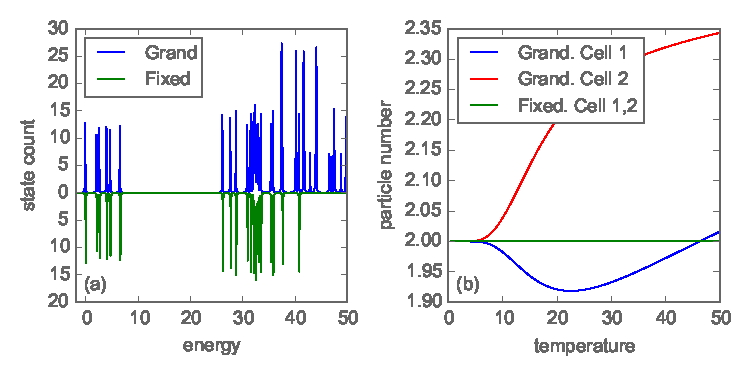
\includegraphics{fixed_charge_approximation}
  \caption{
  (a) Low-energy density of states of the exact grand canonical and the
  approximative fixed charge two-cell QCA system. For small energies the curves
  agree perfectly (up to $E \lesssim 35$). (b) Particle number per cell over
  temperature for the same two-cell system. The curves diverge for $T \gtrsim
  10$.
  }
  \label{fig:fixed_charge_approximation}
  % parameters: V_1 = 100, boa = 2, U = 1000, mu = 250, 2 cells, q = 0
\end{figure}
%
%
\begin{figure}
  \center
  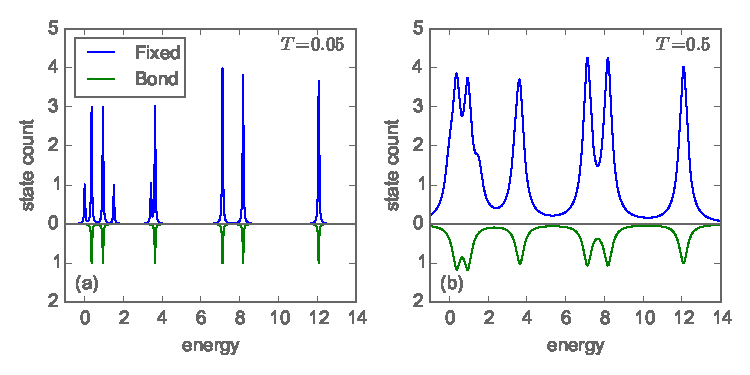
\includegraphics{bond_approximation1}
  \caption{
  (a) Low-energy density of states of a one-cell QCA system for both the fixed
  charge and the bond model. The bond approximation only reproduces the triplet
  states, but omits the singlet states. The ``measurement'' temperature is
  indicated. (b) The same spectrum, but ``measured'' at a higher temperature.
  The singlet-triplet splitting is ``washed out'' at large enough temperatures:
  the singlet and triplet peaks are no longer separately resolved and each bond
  model state corresponds to four fixed charge states at roughly the same
  energy.
  }
  \label{fig:bond_approximation1}
  % parameters: V_1 = 20, boa = 2, U = 1E6, q = 0, P_D = 1, T = 1, mu = 0
\end{figure}
%
The fixed charge approximation is a Hilbert space truncation where we only keep
the states with exactly two electrons per cell.
Fig.~\ref{fig:fixed_charge_approximation}(a) compares the density of states of
the fixed charge model against the exact grand canonical system for a two-cell
system. The chemical potential is $\mu = 250$ and the nearest-neighbour Coulomb
energy is $V_1 = 100$, whereas the on-site Coulomb repulsion is $U = 1000$. The
energies are in units of the hopping $t$, with $t = 1$. The cells are placed a
distance $d/a = 3$ apart, horizontally. This system does not have any
compensation charges, hence $q = 0$. The approximation reproduces the low-energy
spectrum exactly, in the plot up to $E \lesssim 35$. Therefore, as long as the
two-electrons-per-cell sector is lowest in energy and the temperature is small
compared to the energy of the next charge sector, the model works perfectly.
Fig.~\ref{fig:fixed_charge_approximation}(b) plots the number of particles per
cell over temperature and demonstrates the breakdown of the approximation.
Whereas the fixed charge model gives, per definition, a constant number of
particles over the whole temperature range, the grand canonical system's cell
occupancies start to diverge from two electron per cell at around $T \sim 10$.
This roughly corresponds to the energy states the fixed charge model missed at
$E \gtrsim 35$. A small deviation from exactly two electrons per cell is not
detrimental to QCA, a cell occupied by only one or by three electrons, however,
renders QCA non-functional. We often use the fixed charge model as the starting
point and assume, without further investigation, that a practical QCA
implementation can be tuned to be in the right charge regime at a given
temperature.

The bond model neglects doubly occupied states and represents the four states of
a bond---one singlet and three triplets---with only one single bond state. The
model thus assumes that singlet and triplet states are energetically equivalent,
but we had already asserted that we might expect a small singlet-triplet
splitting. Fig.~\ref{fig:bond_approximation1}(a) shows the density of states of
a single QCA cell for both the fixed charge and the bond model. The hopping is
again $t=1$, the nearest-neighbour Coulomb energy is $V_1 = 20$, and the on-site
Coulomb repulsion is $U = 10^6$---practically at infinity. A driver cell placed
at a distance $d/a = 3$ to the left of the single cell sets an input. We have
chosen the driver cell's polarization to be $P_D = 1$. Indeed, each bond state
corresponds to three fixed charge states---the triplet---and one ``close-by''
state---the singlet. They are not energetically equivalent, but split by a small
energy gap, $\Delta E_S$, the singlet-triplet splitting. Like the fixed charge
model, the bond approximation truncates the Hilbert space and the retained
states are exact. Evidently, the bond model keeps one triplet state, but
discards the other two and the singlet. We speculate that, similar to the
antiferromagnetic Heisenberg coupling constant $J$ emerging in the low-energy
limit of the Hubbard model (with $J \sim \frac{t^2}{U}$) \cite{Auerbach}, here,
virtual excitations to high-energy doubly occupied states lower the energy of
the singlet state and make it the ground state. Because the bond model misses
those doubly occupied states, it cannot accommodate singlet states and hence
reproduces the triplet states. Consequently, we cannot hope that the bond model
is correct for ground state and low-temperature properties. We assert that as
long as the singlet-triplet splitting is ``washed out'', that is, as long as the
temperature is much larger than the singlet-triplet gap, $T \gg \Delta E_S$, the
approximation should give good results. At high enough temperatures, the system
no longer ``sees'' the difference between the singlet and the triplet states.
This is illustrated in Fig.~\ref{fig:bond_approximation1}(b) where the spectrum
is ``measured'' at a higher temperature:%
%
\footnote{
We calculate the density of states graphs by folding the energy
eigenvalues of the system---a delta function energy spectrum---with a Lorentzian
with the half-width at half-maximum set by a ``measurement'' temperature. Very
roughly speaking, this corresponds to a photoemission / inverse photoemission
spectroscopy experiment at this temperature.
}%
%
the singlet and triplets are no longer resolved separately. Instead, each bond
state corresponds to four fixed charge states at roughly the same energy.

The figure shows all six bond states of the single cell---the complete spectrum
apart from the doubly occupied states. As this cell is perturbed by a nearby
driver cell with $P_D = 1$, the ground state is qualitatively closest to the
logic 1 state, or $\ket{2}$ in Fig.~\ref{fig:bond}. Similarly, the first excited
state is similar to $\ket{1}$, or logic 0, and the four higher energy states
correspond to $\ket{4}$, $\ket{5}$, $\ket{3}$, and $\ket{6}$, in that order. Of
course, in general the energy eigenstates are a mixture of all basis states, but
we can still characterize them by the most dominantly contributing basis state.
As this a non-charge-neutral system, $q=0$, with a relatively small cell-cell
distance $d/a = 3$, charge buildup tends to push the electrons to the far edge
of the cell, thus making $\ket{4}$ lower in energy than $\ket{6}$.

Since the bond model ignores the singlet-triplet splitting, it is important to
understand how the gap $\Delta E_S$ depends on various system parameters. To
that end we picked out a few selected singlet-triplet states from the spectrum
in Fig.~\ref{fig:bond_approximation1}(a) as examples. Contrary to expectations,
for those states the gap $\Delta E_S$ did not change significantly with the
on-site Coulomb repulsion $U$. However, it did become smaller for shorter and
shorter cell-cell distances $d$. Most importantly, for the nearest-neighbour
Coulomb energy $V_1$ we found $\Delta E \sim \frac{1}{V_1^p}$. The exponent is
$p \sim 3$ when the cell ``sees'' a biasing external potential (e.g.\ $P_D = \pm
1$) and $p \sim 1$ otherwise (e.g.\ $P_D = 0$). Even though our method is
anything but rigorous and the obtained results very likely not universally true,
the findings should nonetheless give a good enough idea of the principle trends.
Quite generally, the higher the overall Coulomb potential---large $V_1$, small
$d$---the smaller the singlet-triplet splitting and, conceivably, the more
accurate the bond approximation. The bond model should work as long as the $T
\gg T_{min}$ with $T_{min} \sim \Delta E_S$, and as a very rough guideline we can
use $\Delta E_S \sim \frac{t^2}{V_1}$. Of course, we also need $T \ll T_{max}$
with $T_{max} \sim U$, so that the doubly occupied states are gapped out.

%
\begin{figure}
  \center
  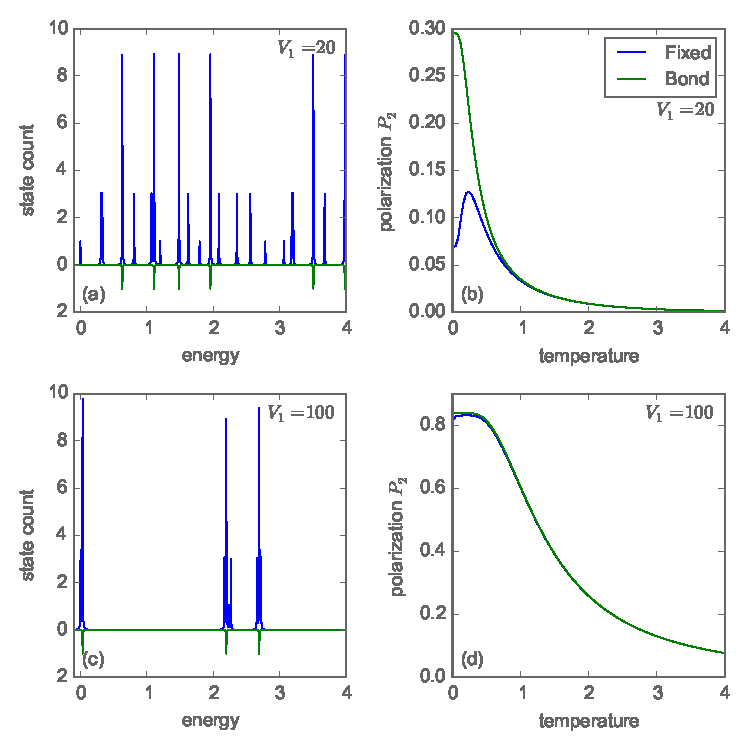
\includegraphics{bond_approximation2}
  \caption{
  The two-cell fixed charge and bond systems at $V_1 = 20$ and $V_1 = 100$.
  (a)(c) Low-energy density of states. (b)(d) Output polarization $P_2$ over
  temperature. For a small Coulomb repulsion the density of states curves look
  qualitatively very different (a) and the bond approximation does not work very
  well (b). At a larger Coulomb repulsion the density of states curves look much
  more alike (c) and the bond approximation works much better (d).
  }
  \label{fig:bond_approximation2}
\end{figure}
%
To illustrate the limitations of the bond approximation we now look at a
two-cell system---a horizontal line of cells with two active cells and a driver
cell to the left. Fig.~\ref{fig:bond_approximation2} shows the spectra and
output polarizations of the system for two different Coulomb energies, $V_1 =
20$ and $V_1 = 100$. Otherwise the parameters are the same as for the one-cell
system in the previous graph. In particular, the spectrum in
Fig.~\ref{fig:bond_approximation2}(a) is exactly the same as in
Fig.\ref{fig:bond_approximation1}(a), except that we have added one more cell to
the system. Each bond state now corresponds to 16 ($4 \cdot 4$) fixed charge
states. Looking at the four lowest-energy peaks in the spectrum, we see that the
bond model exactly reproduces the nine triplet-triplet states, but misses the
three singlet-triplet and the three triplet-singlet states (in the graph the
corresponding two peaks are hardly distinguishable), as well as the single
singlet-singlet ground state. The four lowest bond states should roughly
correspond to, in that order, both cells being aligned with the driver cell (the
ground state), only one of the two cells being aligned with the driver cell, and
both cells being anti-aligned with the driver cell. Higher energy states have at
least one of the cells not in the preferred diagonal states, $\ket{1}$ and
$\ket{2}$, with electrons occupying predominantly the edge of a cell.

Arguably, the spectra of the fixed charge and the bond model in
Fig.~\ref{fig:bond_approximation2}(a) do not look very similar. Consequently,
the polarization curves in Fig.~\ref{fig:bond_approximation2}(b) do not agree,
especially at low temperatures. In fact, it is rather remarkable that given the
widely dissimilar spectra, the polarizations actually do agree relatively well
at higher temperatures, $T \gtrsim 1$. The bond model only reproduces the most
populous energy states of the exact spectrum. Apparently, that is enough to give
(almost) correct results at high temperatures. The lower the temperature, the
more important become the few lowest lying energy states which the bond model
misses. Very roughly speaking, the temperature where the bond model's
polarization becomes accurate also matches the temperature where we saw the
singlet-triplet splitting being washed out in
Fig.~\ref{fig:bond_approximation1}(b). For the much larger Coulomb energy $V_1 =
100$ the spectra look much more alike, qualitatively, even though the bond model
obviously still does not resolve all the lines of the exact density of states,
as illustrated in Fig.~\ref{fig:bond_approximation2}(c). Therefore, the
approximation works much better: the polarization curves agree down to much
lower temperatures and even the discrepancy for the ground state polarizations
is much reduced, as demonstrated in Fig.~\ref{fig:bond_approximation2}(d).
Compared to the $V_1 = 20$ system, the ground state polarization is much larger
and, generally, the higher the cell polarization, the better the agreement
between bond and fixed charge model. We also note that in the spectrum the peaks
are much more spaced out and thus the $V_1 = 100$ wire retains larger cell
polarizations up to much higher temperatures.

The polarization of the fixed charge model shows a curious bump at low
temperatures, for example in Fig.~\ref{fig:bond_approximation2}(b) and
similarly, if less visibly, in Fig.~\ref{fig:bond_approximation2}(d).
Apparently, the ground state is not the most polarized state. Maximum
polarization is reached at a small, but finite temperature. At the same time,
for the bond model the ground state is the most polarized state and generally
its $T=0$ polarization is larger than that of the fixed charge model.
Interestingly, in contrast to the fixed charge model the bond model's ground
state polarization is largely independent of the magnitude of the driver
polarization and also only weakly influenced by the cell-cell distance $d$,
especially for charge-neutral cells where no charge buildup occurs. Instead, it
is predominantly set by $V_1$, and thus by $V_1/t$ and the energy gap $\Delta V
= V_1 - V_0$. Without an external perturbation such as a non-zero driver
polarization the ground state polarization is zero, of course. But any
infinitesimal external perturbation will instantly see the bond model's ground
state become almost fully polarized. We interpret this behaviour as the ground
state actually consisting of two energetically degenerate states, corresponding
to $\pm P_{gs}$, where $P_{gs}$ is the full ground state polarization for a
given $V_1$. The smallest perturbation lifts this degeneracy and sees the system
snapping to either $+P_{gs}$ or $-P_{gs}$. Now the bond model's ground state
corresponds to the fixed charge model's triplet state---one of the lower lying
excited states, but not the ground state. The true ground state of the more
exact model is a single singlet state, a superposition of the $+P_{gs}$ and
$-P_{gs}$ (and other) states. Therefore the polarization of the true ground
state is generally smaller in magnitude than the polarization of the
corresponding two triplet states, explaining the low temperature bump in the
polarization curve and the larger polarization of the bond model's ground state.

%
\begin{figure}
  \center
  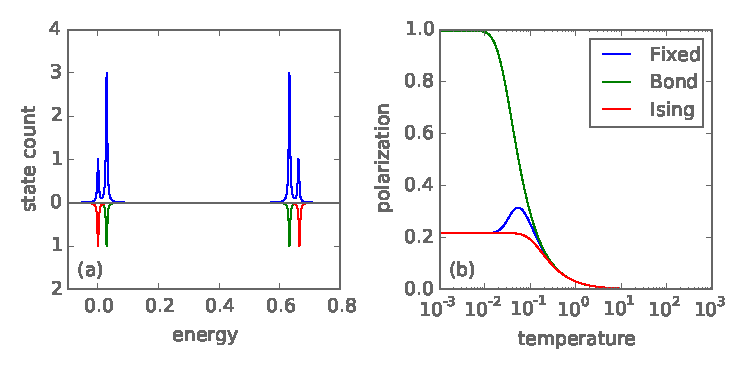
\includegraphics{ising_approximation1}
  \caption{
  Comparing the fixed charge, bond, and Ising model for the one-cell
  charge-neutral QCA system. (a) Low-energy density of states. The Ising model
  reproduces the singlet and not the triplet states, as the bond model does. (b)
  Cell polarization over temperature. At larger temperatures $T \gtrsim 0.3$ all
  three models seem to agree. At $T = 0$ the bond model is wrongly fully
  polarized, whereas the Ising model exactly reproduces the fixed charge model's
  ground state polarization.
  }
  \label{fig:ising_approximation1}
  % parameters: V1 = 100, boa = 3, P_D = 0.1, q = 0.5
\end{figure}
%
The Ising approximation is derived as an effective low-energy model from the
bond Hamiltonian. It is therefore qualitatively different from the previous two
approximations: It is not merely a Hilbert space truncation. \emph{A priori} its
states need not exactly correspond, neither energetically nor qualitatively, to
either the bond or the fixed charge model. Of course, in the limit where the
approximations in the derivation become exact, the Ising model's states should
resemble the bond model's states accurately. Specifically, the derivation
assumed $E \approx V_0$ ($E$ the energy of the whole system) and therefore $t
\ll \Delta V$ as well as $\Delta V \gg T$. The neglected edge states need to be
gapped out. Additionally, cells were assumed to be isolated, so the Ising model
presumably requires reasonably large cell-cell distances. Naturally, the model
inherits the limits of the bond approximation and we would therefore expect $T
\gg \Delta E_S$ ($\Delta E_S$ the singlet-triplet splitting) and $T \ll U$ as
requirements as well. It is important to keep in mind that the Ising model is
not a low-energy model for the more exact fixed charge Hamiltonian---it is
derived as the low-energy limit of the bond model, which, however, is not an
accurate low-energy description of the fixed charge system. The approximation
can also not hope to capture non-charge neutral systems correctly. It simply
lacks the edge states that are the manifestation of charge buildup in non-charge
neutral systems, as discussed in the example of the one-cell bond system above.
We had seen in the derivation of the Ising model that non-charge-neutral cells
are very problematic for the QCA approach in general. Consequently, we will
concentrate on charge-neutral systems, $q = \frac{1}{2}$, for the remainder of
the chapter.

To understand how the Ising approximation behaves we again start by looking at
the density of states for a one-cell system,
Fig.~\ref{fig:ising_approximation1}(a). We have plotted both the fixed charge
and bond models' density of states for comparison and now use slightly different
system parameters: The nearest-neighbour Coulomb energy is $V_1 = 100$, the
cell-cell distance is $d/a = 4$, and the driver cell is only slightly polarized
with $P_D = 0.1$. As always, the hopping is $t=1$. We are in for a surprise!
Evidently, the Ising model reproduces the singlet states and not the bond
model's triplet states. In line with this observation, the Ising model exactly
matches the fixed charge model's ground state polarization, but misses the
triplet-bump at $T \sim 0.05$, Fig.~\ref{fig:ising_approximation1}(b). As a side
note we observe that here, for the charge-neutral system, the bond model's
ground state is fully polarized even at this larger cell-cell distance and for a
very weak driver cell polarization. For the one-cell system the Ising
approximation unexpectedly captures the system's ground state correctly.
Apparently, even though we had derived the Ising model from the bond
Hamiltonian, it does not really resemble the bond model. Instead its states are
of singlet character. In short, the Ising model's behaviour is very confusing.
To lift the confusion, we first note, that even though the Ising model correctly
captures the ground state of the single-cell system, this is not true in
general for larger systems, as we will see in a moment. Second, we need to be
very careful when we talk about the bond model. The bond Hamiltonian is simply a
spinless model that does not distinguish between singlet and triplet states. In
contrast, the bond model uses a concrete basis and we saw that it chooses the
triplet states. Therefore, the bond Hamiltonian, from which we derived the Ising
model, and the bond model are not equivalent. With its choice of basis the Ising
model captures the singlet states. This makes sense in so far as the Ising model
is derived as the low-energy effective model and the singlet states are the
lowest energy states. The Ising and bond model states are therefore different
energetically and qualitatively. Still, in the limit where the Ising model
becomes exact, the singlet-triplet splitting should go to zero and the states of
the two models should become equivalent. On second thought, the fact that the
Ising model exactly reproduces the ground state of the one-cell system is maybe
not as surprising, because we had derived the Ising model precisely for a single
cell.

Close inspection of the energies of the Ising model's only two states as
compared to the energies of the equivalent fixed charge model's states show that
they are not exactly the same. The difference is hardly discernible in the
plotted spectrum, but more pronounced for differently chosen system parameters.
Given that the Ising approximation is an effective model and used several
assumptions in its derivation, this is hardly surprising. For the single-cell
system we can easily study the error of the energies of the Ising states with
respect to the fixed charge states. The states are in better agreement for
larger $V_1$ and smaller $t$. The error explodes for very small cell-cell
distances $d/a < 2$---when the assumption of isolated cells breaks down---but is
largely independent of $d/a$ otherwise. Therefore, we find the assumptions and
limits of the derivation confirmed.

To be able to better quantitatively compare different models we introduce the
relative error of the polarization, defined as
%
\begin{equation}
  \epsilon^I_k = \frac{\left|P^F_k - P^I_k\right|}{P^F_k}
\end{equation}
%
for the Ising model. Here we use the fixed charge model as the reference. Hence,
$P^F_k$ refers to the polarization of cell $k$ with the fixed charge
model and $P^I_k$ is the same polarization, but determined using the Ising
model. The relative error for the bond model, $\epsilon^B_k$, is defined
equivalently. The relative error is independent of the magnitude of the
polarization and therefore suitable for comparing models over a wide parameter
ranges. For best results it is also desirable to not drive the systems
into full polarization. Once cells are saturated at $\left| P_k \right| \sim 1$
the quantitative differences between the models disappear. This is why for our
calculations with the Ising model here, which generally requires larger $V_1/t$
ratios, we have chosen larger cell-cell distances and smaller driver cell
polarizations, resulting in less polarized cells.

%
\begin{figure}
  \center
  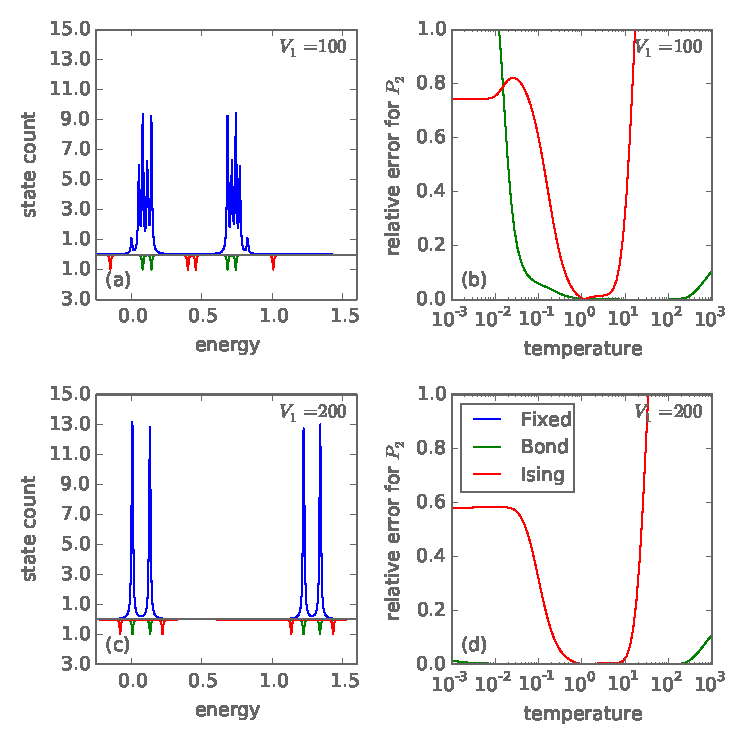
\includegraphics{ising_approximation2}
  \caption{
  Comparing the fixed charge, bond, and Ising model for the two-cell
  charge-neutral QCA system. (a)(c) Low-energy density of states. The Ising
  model's spectrum is qualitatively quite wrong, although it is in better
  agreement with the bond model's spectrum for larger $V_1$. (b)(d) Relative
  error of the output polarization of the bond and Ising model, with respect to
  the fixed charge model. The bond model's error is small over a large range of
  temperatures. At $T \sim U \sim 1000$ the neglected doubly occupied states
  become noticeable. The Ising model's error is small only over a relatively
  small range of temperatures. Its ground state no longer agrees with the fixed
  charge model's ground state.
  }
  \label{fig:ising_approximation2}
  % parameters: V1 = 100, 200, boa = 3, P_D = 0.1, q = 0.5, U=1E3
\end{figure}
%
Fig.~\ref{fig:ising_approximation2} shows the relative error over temperature
together with the density of states for all three models for a two-cell system
at $V_1 = 100$ and $V_1 = 200$. As before we find that the bond approximation
works much better when its spectrum looks qualitatively more similar to the
fixed charge spectrum. At $V_1 = 100$ the bond model yields an almost fully
polarized ground state, whereas the fixed charge model's $T=0$ polarization is
much smaller, resulting in a very large relative error as indicated in
Fig.~\ref{fig:ising_approximation2}(b). At $V_1 = 200$,
Fig.~\ref{fig:ising_approximation2}(d), both fixed charge and bond are almost
fully polarized at low temperatures and the relative error is therefore very
small. For these calculations we used $U=1000$ and indeed we can see that the
bond model starts to diverge for $T \gtrsim 200$. Even at $T=1000$ the error is
relatively small, because the polarization is quite insensitive to doubly
occupied dots, being defined solely as the difference in charge of one diagonal
versus the other diagonal of the cell. At these large temperatures the actual
polarization is already very small.

Looking at the relative error of the Ising model we first notice that it becomes
very large for $T > T_{max}$ with $T_{max} \sim 5 \ldots 10$. Of course, this is
a consequence of the Ising model missing the gapped out edge states, where the
gap is $\Delta V \sim 0.3 V_1$. Accordingly, $T_{max}$ is larger for $V_1 = 200$
than for $V_1 = 100$, though maybe not by as much as we might expect. In stark
contrast to the one-cell system, for two cells the Ising model's ground state no
longer agrees with the ground state of the fixed charge model. The Ising $T=0$
polarization is generally smaller than the polarization of the more exact model.
Similarly to the bond model, the relative error of the ground state polarization
decreases for increasing $V_1$. We never expected the Ising model to get the
low-temperature behaviour right and in this light, the surprising agreement of
the ground state for the one-cell system can be viewed as a curious coincidence,
related to the details of how exactly we had derived the Ising model. The
relative error curves of the Ising model reveal that the temperature range where
the error is actually small---that is, where the Ising model can be considered
valid---is quite narrow. For $V_1 = 100$ it is almost like a sweet spot, a very
narrow window around $T \sim 1$. For $V_1 = 200$ the situation is much better,
the error is close to zero in the temperature range $T = T_{min} \ldots T_{max}
\sim 0.8 \ldots 8$. This temperature range only very weakly depends on the
cell-cell distance $d/a$ or the driver polarization $P_D$. It is dominantly set
by $V_1$. Roughly speaking, the lower temperature limit $T_{min}$ is set by the
singlet-triplet splitting, which becomes smaller with increasing $V_1$, and the
upper temperature limit $T_{max}$ is set by $\Delta V$ which is, of course,
directly proportional to $V_1$. Here we have, as always, kept the hopping
constant at $t=1$. In agreement with our analysis for the one-cell system, the
relative error at a fixed temperature decreases with increasing $V_1$, but is
largely independent of $d/a$ as long as $d/a$ is not too small.

The spectra of the Ising approximation do not compare well with the fixed charge
or bond model, especially at $V_1 = 100$. Clearly, the Ising model gets the
energy levels completely wrong. However, we have to keep in mind that, in
contrast to the bond model, the Ising model's states may be qualitatively
different from the more exact models' states. Therefore, even though the
spectrum looks completely wrong, the Ising model still does work correctly, if
in a very small temperature range. In the right limit the Ising model should
eventually resemble the bond model and accordingly, at $V_1 = 200$, the two
models' spectra do look more agreeable. The qualitative agreement of the spectra
becomes better for smaller cell-cell distances and larger driver cell
polarizations as well, thus generally when the cells are more fully polarized.

All told, the Ising model is a tricky approximation. It is conceptually
confusing, because, even though it is derived from the bond Hamiltonian, it does
not exactly resemble the bond model. Adding to this confusion is the fact that
it gets the ground state of the one-cell system right. From a practical point of
view, the Ising model requires very large $V_1/t$ ratios and its operational
window can be very small. Great care should be exercised when using the Ising
approximation for calculations. They should be verified with a more exact model
as much as possible and the error, and trends of the error, should be kept in
check. Where an explicit verification is not possible, for larger systems, its
result should be taken with a grain of salt.

As a final step we look at a few concrete systems and their error trends. For a
horizontal line of cells with three to five cells with a cell-cell distance of
$d/a = 4$ and a nearest-neighbour Coulomb energy $V_1 = 100$,
Fig.~\ref{fig:ising_approximation3}(a) shows the relative error as a function of
the number of cells in the system. For these larger systems the Ising
approximation and its error are benchmarked against the bond model and not the
fixed charge model as before. We notice that for these wires the error is quite
a bit smaller at $T = 2$ compared to $T = 1$, and 1\% error seems to be the best
we can do. Most worryingly, the error increases with the number of cells in the
wire. This trend holds quite generally, for a range of systems with different
cell-cell distances $d/a$ and Coulomb energies $V_1$. Consequently, we expect
the error to grow with increasing system sizes and once the systems are too
large for bond model calculations we will not be able to give a good upper error
bound. The error will become uncontrolled. On a slightly more optimistic note,
the error seems to decrease from cell to cell inside each wire. This is explored
in more detail in Fig.~\ref{fig:ising_approximation3}(b), where we have plotted
the error of each cell inside a five-cell wire. Evidently, the error decreases
along the wire and we can expect this decrease to counter the generally growing
error for longer and longer wires, at least as long as we are mainly interested
in the output polarization of the wire. This trend is not true generally and for
differently chosen system parameters the error may also remain constant along
the wire. Still, for this particular QCA structure for the chosen system
parameters we are relatively confident that the error of the output
polarization, while not well controlled, will not grow very large for systems
accessible with the Ising approximation---up two twelve QCA cells. 
%
\begin{figure}
  \center
  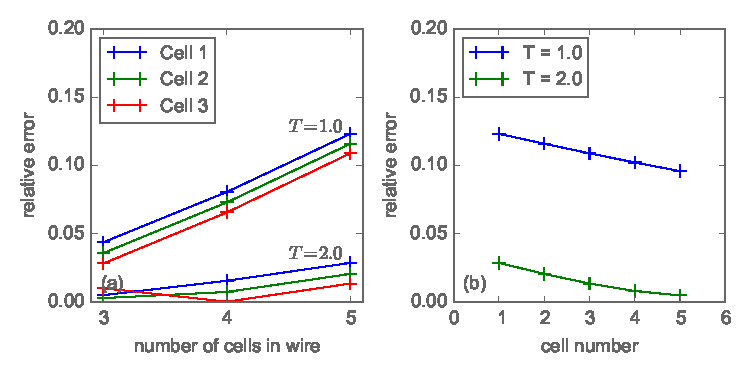
\includegraphics{ising_approximation3}
  \caption{
  (a) The Ising model's relative error of the cell polarization for three-cell
  to five-cell charge-neutral wires at two different temperatures. The longer
  the wire the larger becomes the error. The error is no longer well controlled.
  (b) The Ising model's relative error for each cell's polarization in a
  five-cell charge-neutral wire. For the chosen parameters the error decreases
  along the wire. At least for the output polarization the effect of a growing
  error with increasing wire length is therefore countered.
  }
  \label{fig:ising_approximation3}
  % parameters: V1 = 100, boa = 3, P_D = 0.1, q = 0.5; 5 cells
\end{figure}
%

In this chapter we introduced and established three approximations for QCA
systems, the fixed charge, the bond, and the Ising model. We usually use the
fixed charge model as the starting point, without further explicit verification.
In principle, whether the fixed charge approximation holds for some chosen set
of parameters has to be checked for each potential QCA implementation on a case
by case basis. If the fixed charge model is not applicable, then there is also
generally no hope of implementing QCA on the given experimental system. We
generally assume doubly occupied states to be sufficiently gapped out and put
$U$ at infinity. The bond approximation is then a very good description of QCA
systems at high temperatures. It starts breaking down when the temperature
becomes comparable to the singlet-triplet splitting and therefore for small
$V_1$ and too large cell-cell distances. While it is conceptually deeply
rewarding to map QCA to an Ising system, we have seen the Ising approximation to
be difficult to handle and control for practical calculations. It is only valid
in a relatively small parameter window and great care has to be taken with its
application. Generally speaking, both the bond and the Ising approximation
become exact in the same limits---large $V_1/t$ and small (but not too small)
cell-cell distances. Not coincidentally, those are the limits where the QCA
approach works best. Both approximations are useless for low-temperature
calculations and for ground state properties we thus have to rely on the fixed
charge model, which, however, only allows system sizes of up to three cells. We
will use the bond model for most of our QCA characterization work at finite
temperature. With system sizes of up to six cells it already allows for some
interesting insights. The Ising model is problematic and we will employ it
sparingly and only to look at larger structures such as gates.

% TODO: Include partition function argument / explanation somewhere?
% TODO: good argument why there are two degenerate ground states for the bond
% model? (triplet, symmetry argument?)
% TODO: Is there a better explanation why bond chooses triplet and Ising singlet
% states?
% TODO: mention two sets of conditions (energy gap and temperature related) for
% Ising model?
% TODO: maybe explain somewhere: Ising weirdness is not a shortcoming of our
% derivation, but a consequence of pressing QCA in a two-state basis


\bibliography{bibliography}{}
\bibliographystyle{utcaps}

\end{document}
